\chapter{A Deep Learning Pipeline for Pennycress Seed Pod Phenotyping}\label{ch2:pennycress}
\section{Introduction}\label{sec:ch2-pc-background}
Pennycress (\textit{Thlaspi arvense L.}) is a winter annual in the \textit{Brassicaceae} family that has shown potential as a bioenergy feedstock and cover crop due to its winter-annual habit, growth in the fallow period, and amenability to genetic modification \cite{moser2009production,sedbrook2014new}. Its short generation time, established transformation protocols, sequenced reference genome \cite{nunn2022genome} and species-wide pangenome \cite{bird2026pangenome} make pennycress a viable candidate for breeding and domestication \cite{sedbrook2014new}. However, domesticating pennycress requires improving yield, seed retention, and cover-crop/feedstock traits \cite{sedbrook2014new}. In \textit{Brassicaceae}, silicle morphology is directly tied to seed yield and pod shattering \cite{nichol2025shock}. Pods play an active role in development and resource allocation, not merely containing seeds \cite{wing-seed-assoc}. Pod walls are photosynthetically active and supply assimilate to the developing seed \cite{hua2012silique,zhu2018silique}. Seeds per pod is one of three multiplicative components of seed yield, alongside pods per plant and seed weight, and in rapeseed its natural variation is under maternal and embryonic genetic control \cite{zhu2020seednumber}. Therefore, tissue-specific pod traits such as wing area, envelope area, seed count, and tissue-to-seed ratios are biologically meaningful targets for breeding and phenotyping.

However, realizing the potential of pennycress as a biofuel feedstock requires population-scale studies characterizing variation in feedstock-relevant traits, which are currently limited by phenotyping bottlenecks, most notably the manual collection of pod-level traits \cite{li2014review,seed-cnn}. Although high-throughput methods exist for measuring seed composition \cite{tuite2025nirs}, single-seed weight \cite{clohessy2018singleseed}, and seed shape \cite{tanabata2012smartgrain}, each operates on individual seeds and extracts a limited set of traits. These techniques do not resolve distinct pod tissues (wing, envelope, and seed) or support the depth of morphological and inter-tissue measurements that pod-level phenotyping requires. Despite their relevance to pennycress improvement, pod traits have not been measured at tissue resolution across large pennycress panels.

The central bottleneck to measuring pod traits is tissue segmentation, which requires separating wing, envelope, and seed regions, and counting seeds in each pod \cite{seed-cnn}. This process is labor-intensive because each pod requires boundary tracing, object separation, and visual inspection \cite{li2014review}. Consequently, manual measurement limits both sample size and trait depth, forcing researchers to measure either fewer accessions or fewer traits \cite{seed-cnn}. As a result, detailed pod traits are systematically omitted from population-scale studies. Automated segmentation addresses this bottleneck by converting raw images into tissue-specific masks that can be used for scalable trait extraction \cite{li2014review, lagergren2023fewshot}.

In other domains, image-based phenotyping has enabled measurements at scales and resolutions that are infeasible by hand, from cell-level microscopy to satellite imagery \cite{li2014review,lagergren2023fewshot}. A single imaging modality can yield many traits simultaneously, allowing researchers to extract complex topological and morphological features that are inaccessible with manual measurement \cite{li2014review}. For pod-level phenotyping, the operative task is segmentation, which separates wing, envelope, and seed regions within each pod. Classical segmentation approaches require controlled imaging conditions and manually tuned thresholds, which do not generalize across natural variation in raw scans.

Unlike classical segmentation, deep learning models operate on raw images directly, learning relevant features end-to-end; deep learning has achieved state-of-the-art performance across computer vision tasks \cite{krizhevsky2012imagenet, he2016deep}. In the plant phenotyping domain, deep learning models have been applied to disease detection \cite{mohanty2016plantdisease}, organ counting \cite{ubbens2018leafcounting}, seed-per-pod estimation \cite{seed-cnn}, and population-scale trait extraction \cite{wang2019high,lagergren2023fewshot}. In particular, convolutional neural networks (CNNs) learn hierarchical filters over local image neighborhoods \cite{lecun2015deep}, giving them a spatial inductive bias well suited to segmentation. U-Net is a CNN-based segmentation architecture that shows strong performance on small, specialized biological and biomedical segmentation tasks, making it a natural baseline for tissue-level pod segmentation \cite{unet}. More recent architectures can improve performance in some settings but may require larger datasets, different preprocessing, or task-specific adaptation. Because pennycress pod segmentation is a small, specialized biological task with fine seed/envelope boundaries, benchmarking modern architectures against U-Net is necessary.

Once tissue-resolved pod traits can be measured at scale, the next challenge is linking trait variation to candidate genetic mechanisms. High-throughput phenotyping can be used in conjunction with genome-wide association studies (GWAS) \cite{uffelmann2021genome} to reveal the genetic architecture of phenotypes, providing candidate genes and markers for breeding. A network-based framework that leverages multiple lines of evidence in pennycress or related species utilizes GRIN (Gene set Refinement through Interacting Networks) \cite{sullivan2024grin}, \textsc{Mentor} (Multiplex Embedding of Networks for Team-Based Omics Research) \cite{mentor}, and \textsc{Mentor-IA} (\textsc{Mentor} Interpretation Agent) \cite{mentor-ia} to prioritize these candidates and resolve them into interpretable modules, yielding candidate mechanisms. This framework has been applied to other pennycress traits \cite{combsgiroir2024waterlogging}, but not to intensive, tissue-resolved pod phenotypes in pennycress.

In this work, we developed a deep learning pipeline for pennycress seed pod segmentation, enabling deep, tissue-resolved phenotyping at population scale. We benchmarked a suite of modern computer vision models, spanning CNNs, vision transformers, and foundation models. We found that a custom U-Net provided the most efficient pod tissue segmentation performance with comparable accuracy to modern models and a 30- to 45-fold speed increase over manual phenotyping. We applied this pipeline at population scale to over 12,000 pods from 768 accessions and used it to identify candidate loci, genes, and mechanisms underlying pod traits.

\section{Materials and Methods}
\subsection{Experimental Design}
We designed this study to explore whether it was possible to use deep learning to accelerate image-based pennycress pod phenotyping and connect the extracted phenotypes to candidate genetic mechanisms for pennycress improvement. Following this objective, our study contains two main components. In the first stage, we trained and benchmarked a U-Net segmentation model to extract 52 per-pod phenotypes, applied the model at population scale to 12,253 pods, and examined the resulting trait matrix for biological coherence with a predictive phenotype network. In the second stage, we filtered traits by heritability ($H^2 \geq 0.05$), connected them to loci via GWAS (significant at $p < 1 \times 10^{-6}$), and mapped loci to candidate genes. We then pruned the candidates with GRIN and resolved the survivors into modules with \textsc{Mentor}. With the assistance of \textsc{Mentor-IA}, we interpreted the modules to generate exploratory mechanistic hypotheses for genetic targets. Our data were sourced from a 768-accession panel of pennycress pod images, collected from field sites in the midwestern United States. Broad-sense heritability was estimated on $n=25$ replicated genotypes, and GWAS was performed on a subset of 189 genotyped accessions from dryland environment treatments.

\subsection{Dataset}\label{sec:ch2-pennycress-dataset}
\subsubsection{Data Collection}
Our raw data consisted of 768 scanned images of pennycress (\textit{Thlaspi arvense L.}) seed pods collected from field sites in the Midwest, including those at Western Illinois University (WIU), Illinois State University (ISU), and University of Minnesota (UM). After collecting seed pods, we imaged them using an Epson V39 Perfection scanner. Each scanned image contained multiple seed pods due to their size. Figure~\ref{fig:ch2-pennycress-scan-annotation}A displays an example raw image scan. The 768 scans represented 768 pennycress accessions, with each scan typically containing approximately 10--20 seed pods.

\subsubsection{Data Annotation}\label{sec:ch2-annotation}

For supervised model training, we created pixel-level annotations using GNU Image Manipulation Program (GIMP). We labeled three areas of each pennycress seed pod: the wing was annotated with red pixels, the envelope was annotated with green pixels, and the seeds were annotated with blue pixels. We annotated these areas due to the biological significance of their phenotypes. Figure~\ref{fig:ch2-pennycress-scan-annotation}B and C show an example of a separated pennycress seed pod and its associated segmentation. We manually annotated 21 scanned images, amounting to 347 annotated seed pods. We assigned 16 scans containing 282 pod crops to the development set and reserved 5 scans containing 65 pod crops as an independent test set used only for final benchmarking. Within the development set, we randomly allocated the 282 pod crops in an 80:20 ratio to training and validation subsets, respectively. The validation subset was used for checkpoint selection and early stopping; the independent test set was not used during training or checkpoint selection and was evaluated only for the final architecture benchmark.

\begin{figure}[!ht]
 \centering
 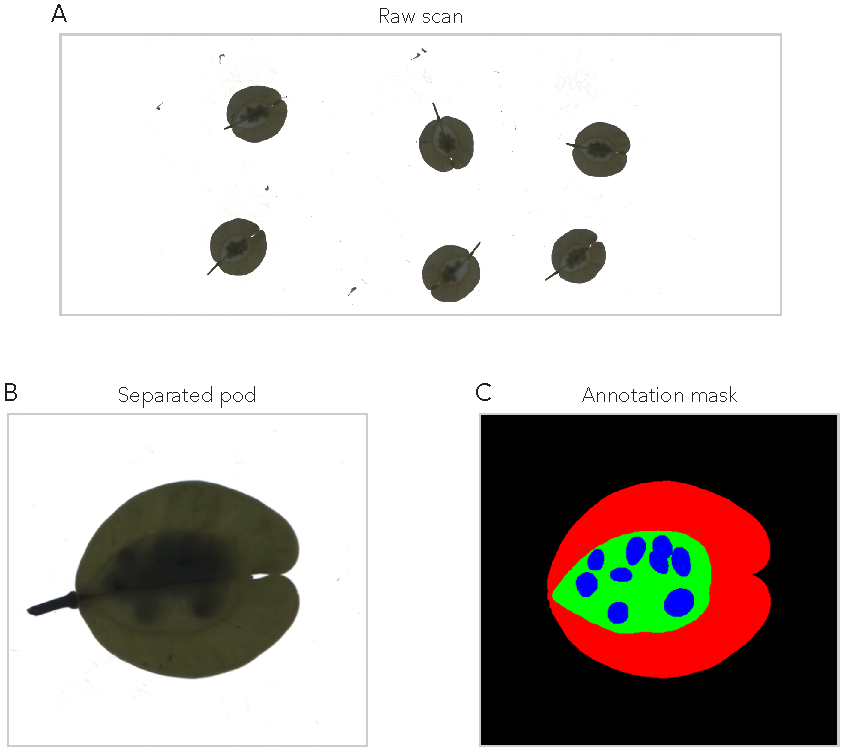
\includegraphics[width=\linewidth]{figures/pennycress-unet/pennycress_scan_annotation.pdf}
 \captionsetup{justification=raggedright,singlelinecheck=false}
 \caption[Raw pennycress seed-pod scans and pixel-level annotations.]{Raw pennycress seed-pod scan, separated pod crop, and pixel-level annotation. (A) Flatbed scan excerpt showing multiple \textit{Thlaspi arvense} seed pods on a white scanner background before object separation, annotation, and segmentation preprocessing. (B) Separated \textit{T. arvense} seed pod extracted from a raw scan. (C) Corresponding semantic annotation mask, with wing tissue in red, envelope tissue in green, seeds in blue, and background in black.}
 \label{fig:ch2-pennycress-scan-annotation}
\end{figure}

\subsubsection{Data Preprocessing}\label{sec:ch2-preprocessing}
Before model input, we separated each pennycress seed pod in the raw image. We created rectangular bounding boxes around each seed pod object in Python, and we saved each bounding box as a separate image, yielding a dataset of 12,253 individual pods across the 768 scans. We used these separated images for model input.

\subsubsection{Image Tile Generation}\label{sec:ch2-tile-gen}
We implemented a tile generation scheme to increase the amount of training data available and build an invariance to common imperfections that occur during the image collection process. Tiling is a form of image augmentation that divides each image into small, fixed-size patches that serve as training examples.

Prior to tiling, we padded each separated image with 128 pixels in all directions. Image padding enables us to generate tiles near the edge of images, allowing the model to see a greater context. The red box in the leftmost image in Figure~\ref{fig:ch2-pennycress-preproc} highlights the padding boundary, and the remaining panels show the corresponding semantic and class-specific masks used during tile sampling. While we also used a tile size of 128 pixels, the padding and tile size are independent parameters.

After padding, we selected a tile size of 128 pixels. Pixels on the seed pod were randomly initialized as tile centers. After the algorithm selected center pixels, it used the surrounding 128 $\times$ 128 pixels to create each tile.

\begin{figure}[!ht]
 \centering
 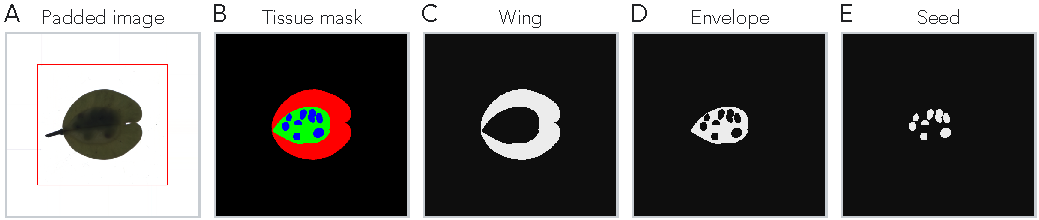
\includegraphics[width=\linewidth]{figures/pennycress-unet/pennycress_preprocessed_images.pdf}
 \captionsetup{justification=raggedright,singlelinecheck=false}
 \caption[Preprocessing outputs for model training.]{Preprocessing outputs for model training. (A) Padded separated pod image; the red rectangle marks the original crop boundary after adding 128 pixels of context on each side. (B) Full semantic tissue mask. (C--E) Binary masks for wing, envelope, and seed classes, respectively.}\label{fig:ch2-pennycress-preproc}
\end{figure}

During validation, we left tiles unchanged to prompt the most accurate predictions possible. However, during training, we applied various image augmentations and transformations to build an invariance to common data collection issues. We applied rotation, blur, saturation, brightness, flips, and transposes with a 50\% chance of occurrence each, greatly increasing the number of unique types of tiles that could be generated.

We selected each type of transformation to combat certain issues that occur during the scanning process. For example, blur transformations simulate potential smudges on the scanner screen. Rotations model the differences in angle between scanned seed pods, and brightness transformations capture the potential for shadows underneath folds in an image. By using these transformations to simulate real imaging issues, the model learns to become invariant to such features and instead focus on biologically relevant information. Therefore, the tile generation scheme serves two purposes. It increases the amount of available training data, and it builds an invariance to common scanning issues. We show examples of generated training tiles, their corresponding labels, and representative augmentation outputs in Figure~\ref{fig:ch2-tile-gen-ex}.

\begin{figure}[!ht]
 \centering
 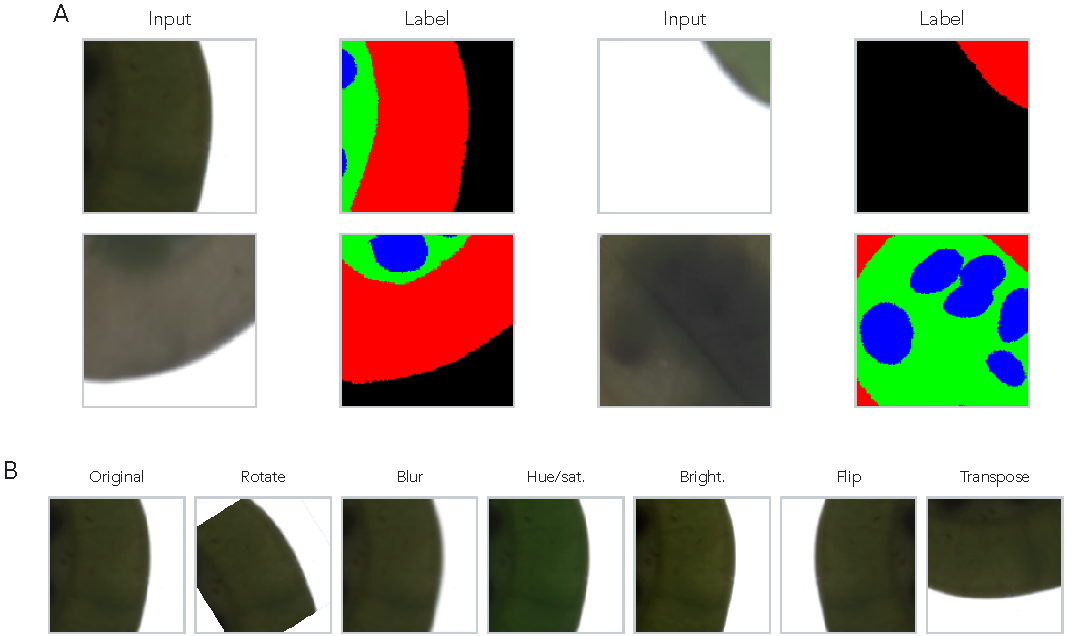
\includegraphics[width=\linewidth]{figures/pennycress-unet/tile_gen.pdf}
 \captionsetup{justification=raggedright,singlelinecheck=false}
 \caption[Example training tiles and augmentation outputs.]{Example training tiles and augmentation outputs. (A) Input and label pairs show 128$\times$128 tiles sampled from padded seed-pod images and their corresponding tissue-label masks. Tiles include background, pod-boundary, tissue, and seed contexts used for model training. (B) Representative image-tile augmentations show the transformation families applied during training, including affine rotation, blur, hue/saturation shift, brightness/contrast adjustment, flip, and transpose operations.}\label{fig:ch2-tile-gen-ex}
\end{figure}

\subsection{U-Net Baseline}\label{sec:ch2-unet}
\subsubsection{Architecture}
We used U-Net \cite{unet}, a fully convolutional encoder-decoder architecture in which a contractive path captures hierarchical context and a symmetric, expansive path recovers spatial localization. We adapted the original architecture with a modified block structure, SELU activations, and tuned hyperparameters for tissue-level pod segmentation.

Because raw seed pod images were too large and computationally expensive to fit into model memory while training, we used the generated tiles created in Section~\ref{sec:ch2-tile-gen} for training.

The model's input is a 3-channel RGB tile of size 128 $\times$ 128, and its output is also 128 $\times$ 128 with four channels corresponding to background, wing, envelope, and seed classes. We applied a softmax activation function to create a pixel-wise segmentation map, where the model gives each pixel a class label. We then compared segmentation maps to the corresponding hand-annotated segmentations detailed in Section~\ref{sec:ch2-annotation} and minimized the weighted cross-entropy loss between them to train the model.

The main component in the U-Net architecture is a convolutional block. Each block contains three convolutional layers with 3 $\times$ 3 kernels; each convolution is followed by batch normalization, SELU activation, and dropout with a rate of 0.1.

The network comprises nine convolutional blocks (Figure~\ref{fig:ch2-pennycressunet}), beginning with a 32-kernel block at the full 128$\times$128 tile resolution. The four contractive blocks are separated by 2$\times$2 max-pooling that halves spatial resolution while increasing the channel depth from 32 to 256. A 512-kernel bottleneck operates at 8$\times$8 resolution. The four expansive blocks reverse this with upsampling-convolution steps that restore spatial resolution and reduce channel depth, returning to 128$\times$128. Skip connections concatenate contractive and expansive feature maps, improving gradient flow and fusing features across scales. A final 1$\times$1 convolution produces the four-channel segmentation map.

\begin{figure}[!ht]
 \centering
 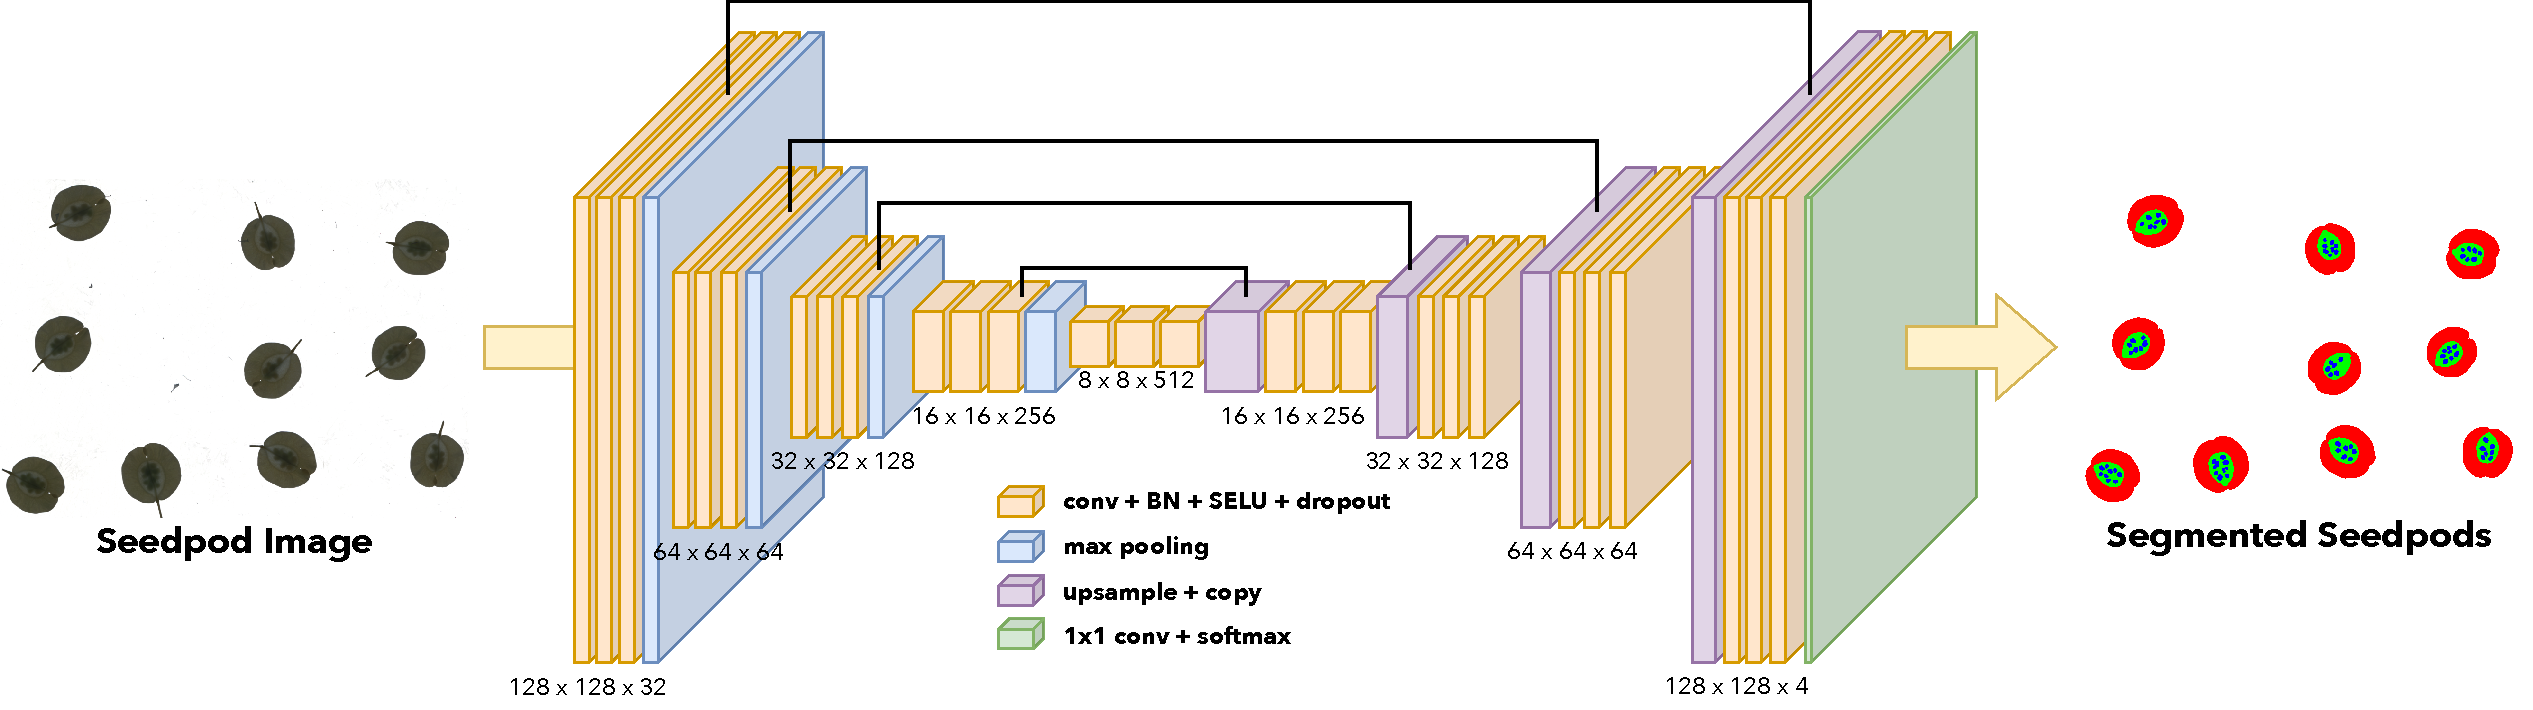
\includegraphics[width=\linewidth]{figures/pennycress-unet/PennycressUNet.pdf}
 \captionsetup{justification=raggedright,singlelinecheck=false}
 \caption[Pennycress U-Net architecture]{Pennycress U-Net architecture. The model takes a 128$\times$128 RGB seed pod tile as input and returns a 128$\times$128 four-channel semantic segmentation map for background, wing, envelope, and seed classes. Orange blocks denote 3$\times$3 convolution, batch normalization (BN), SELU activation, and dropout; blue blocks denote max pooling; purple blocks denote upsampling with skip-copy connections; and the green block denotes the final 1$\times$1 convolution with softmax output. Feature-map labels are shown as height $\times$ width $\times$ channels.}
 \label{fig:ch2-pennycressunet}
\end{figure}

\subsubsection{Boundary-Weighted Cross Entropy Loss}
To account for uncertainty in the exact boundaries of our ground-truth labels, we implemented a weighted cross-entropy loss that scales the per-pixel loss by a boundary-aware weight map.

We first compute a raw weight map from the eroded seed mask. We binarize the seed channel, subtract its binary erosion to isolate the boundary ring, and then calculate the Euclidean distance from each pixel to the closest border pixel to produce a distance map. We clip distances at a maximum of $b = 5$ pixels and normalize to the range $[0, 1]$. We evaluated two configurations parameterized by a border weight $w_b$.

In the \textbf{boundary down-weighted} configuration ($w_b < 1$), we min-max normalize the raw weight map so that pixel values $W_{i,j} \in [0, 1]$, where $i$ and $j$ index the row and column of a pixel within a tile. We then invert the weight map so that pixels with a smaller distance to the boundary have a lower weight value. Finally, we scale the weight map so that its range is $W_{i,j} \in [w_b, 1]$. This configuration treats boundary annotations as the noisiest signal and lets the model rely more on confidently-labeled interior pixels.

In the \textbf{boundary up-weighted} configuration ($w_b > 1$), we instead clip the raw weight at a minimum of $1$, yielding $W_{i,j} \in [1, w_b]$ so that distant pixels carry weight $1$ and boundary pixels carry weight up to $w_b$. This configuration treats boundaries as the most informative regions to learn.

We then multiply the weight map pixelwise with cross-entropy loss and average over pixels:

\begin{align}\label{eq:ch2-wce}
 L_{WCE}(t, p(\theta)) = - \frac{1}{\mid I \mid \mid J\mid} \sum_{j}^{J} \sum_{i}^{I} \sum_{k}^{K} W_{i,j} (t_{i,j,k} \log(p(\theta)_{i,j,k})),
\end{align}

\noindent where $t$ is the ground truth segmentation map and $p(\theta)$ is the predicted segmentation map as a function of U-Net parameters. The indices $i$ and $j$ run over the $I$ rows and $J$ columns of a tile, so $\mid I \mid \mid J \mid$ is the number of pixels the loss is averaged over, and $k$ runs over the $K = 4$ classes (background, wing, envelope, and seed). For a given pixel, $t_{i,j,k}$ is $1$ if that pixel is labeled class $k$ in the ground truth and $0$ otherwise, while $p(\theta)_{i,j,k}$ is the softmax probability the model assigns to class $k$ at that pixel. The inner sum over $k$ therefore reduces to the log-probability the model placed on the correct class, and $W_{i,j}$ rescales that pixel's contribution according to its distance from a seed boundary.

\subsubsection{Model Training}
We trained the U-Net for up to 150,000 mini-batch updates using the Adam optimizer with a batch size of 32. Rather than partitioning training into fixed epochs over the tile dataset, we sampled tiles continuously from the train split (Section~\ref{sec:ch2-pennycress-dataset}) and tracked progress by iteration count. We evaluated validation loss every 1,000 batches and applied an early stopping criterion of 50 evaluation intervals. If the best validation loss did not improve over 50 consecutive checkpoints (50,000 batches), training terminated.

We used a learning rate schedule with linear warmup and cosine decay. The learning rate ramped from 0 to $1\!\times\!10^{-3}$ over the first 1,000 batches to stabilize early gradients, then decayed via a cosine schedule to $1\!\times\!10^{-5}$ over the subsequent 90,000 iterations and held constant thereafter.

\subsection{Phenotype Extraction}\label{sec:ch2-phenotype-extraction}

We developed functions to extract 52 features from each seed pod segmentation map, grouped into three categories: absolute, ratio, or color.

\subsubsection{Absolute Features}

We calculated seven absolute features from each segmentation map: wing area and perimeter, envelope area and perimeter, seed area and perimeter, and seed count. Areas for each tissue were calculated by summing the pixels assigned to that class. Perimeters were calculated using Scikit-Image~\cite{scikit-image} on nested binary masks. Wing perimeter was calculated from the union of wing, envelope, and seed pixels, envelope perimeter was calculated from the union of envelope and seed pixels, and seed perimeter was calculated on the raw (pre-watershed) seed mask, giving the total boundary length of all seed pixels in the pod. Pixel counts were converted to physical area by dividing by DPI$^2$ ($600^2=360,000$) and multiplying by 6.4516 cm$^2$/in$^2$.

In addition to measuring area and perimeter features, we utilized the watershed algorithm to count the number of seeds in each segmented image. First, we isolated the seed channel and applied a morphological opening to suppress noise. Then, we calculated the Euclidean distance from each seed pixel to the nearest non-seed pixel. We applied a threshold to this distance map, setting any pixel that was less than 60\% of the maximum distance value in the map to 0. The thresholded foreground was labeled into connected components and passed as markers to the OpenCV~\cite{opencv_library} watershed algorithm, which returned a per-seed segmentation; seed count is defined as the number of unique markers in the map. The watershed process is visualized in Figure~\ref{fig:ch2-watershedding}.

\begin{figure}[!ht]
 \centering
 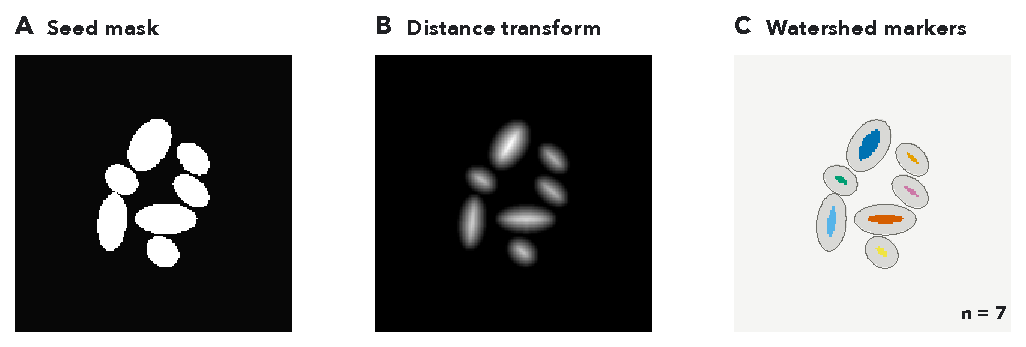
\includegraphics[width=\linewidth]{figures/pennycress-unet/watershedding.pdf}
 \captionsetup{justification=raggedright,singlelinecheck=false}
 \caption[Seed-count extraction by watershed segmentation]{Seed-count extraction by watershed segmentation. (A) Binary seed mask isolated from the U-Net segmentation map. (B) Euclidean distance transform used to identify seed interiors. (C) Connected-component markers after thresholding the distance map at 60\% of its maximum value; colors denote marker identities used to initialize watershed segmentation, and the resulting marker count defines seed count.}
 \label{fig:ch2-watershedding}
\end{figure}

\subsubsection{Ratio Features}
We calculated 18 ratio features from the segmented seed pod masks, with six to-total ratios and twelve between-tissue ratios, evenly split between area and perimeter-based variants. The six to-total ratios divide each tissue's area or perimeter by the total area or perimeter, yielding wing-to-total, envelope-to-total, and seed-to-total ratios for both measurement types.

The 12 between-tissue ratios cover all pairs of distinct tissues for both area and perimeter. These include ratios into seed (envelope/seed, wing/seed), into envelope (wing/envelope, seed/envelope), and into wing (seed/wing, envelope/wing), computed for both measurement types. Reciprocal ratios are retained (e.g., seed/envelope and envelope/seed) so that downstream analysis is not restricted.

\subsubsection{Color Features}
We extracted nine color features from each tissue: red, green, blue (RGB); hue, saturation, brightness (HSV); and lightness, $a^*$ (green-red), and $b^*$ (blue-yellow) from CIELAB. We converted each input image into all three color spaces using OpenCV~\cite{opencv_library}. We then created a tensor of these features with size $\texttt{height} \times \texttt{width} \times 9$. We used the segmentation masks to subset this tensor by tissue, yielding three sub-tensors covering wing, envelope, and seed features separately.

We aggregated each color channel across spatial dimensions by taking the mean over the relevant tissue's pixels, producing a nine-dimensional color vector per tissue. Across the three tissues, this yielded 27 features in total.

\subsection{Segmentation Architecture Benchmarking}\label{sec:ch2-benchmark}
To ensure that our pipeline extracts the most accurate downstream phenotypes possible, we identified the most effective segmentation architecture. We tested six architectures across three families: CNNs, transformers, and foundation models.

We compared two CNN architectures to the baseline U-Net: nnU-Net \cite{isensee2021nnu} and DeepLabV3+ \cite{chen2018encoder}. nnU-Net is an approach that configures a U-Net systematically through a three-stage pipeline. The selection process includes fixed parameters that generalize across many datasets; rule-based parameters that are determined by unique dataset and pipeline characteristics; and empirical parameters that are learned through trial and error. Because nnU-Net derives its own patching, batch size, and augmentation scheme through fingerprinting and rule-based selection, the benchmarking for this architecture did not include our custom tile generation scheme (Section~\ref{sec:ch2-tile-gen}). DeepLabV3+ combines an encoder-decoder architecture with atrous depthwise separable convolutions, balancing the use of long-range spatial context with fine-grained boundary detection.

We selected SegFormer \cite{xie2021segformer} and Mask2Former \cite{cheng2022masked} as exemplar transformer architectures for benchmarking. SegFormer uses a hierarchical transformer encoder backbone that generates both high-resolution, fine-grained features and low-resolution, coarse features, and a lightweight MLP decoder to fuse these features for the final semantic segmentation task. Unlike SegFormer, which optimizes a per-pixel classification objective, Mask2Former adopts an alternate paradigm based on set prediction. Mask2Former uses a multi-scale encoder backbone to extract features, which are then upsampled to high-resolution per-pixel embeddings with a pixel decoder. Additionally, Mask2Former utilizes a transformer decoder with learnable query inputs to predict mask candidates. These queries are refined through cross-attention with the multi-scale features, and the transformer decoder output and pixel decoder output are combined via dot product to produce region predictions. Although Mask2Former is designed to be a general segmentation architecture, supporting panoptic, instance, and semantic segmentation, we trained only for a semantic segmentation objective due to our task formulation.

We evaluated SAM 3 \cite{carion2025sam3} as a candidate foundation model for benchmarking. SAM 3 is a foundation model designed for promptable concept segmentation, taking input as either text or image exemplars. SAM 3 was trained with a model-in-the-loop data engine on over 1 billion images, generating segmentation examples using human input while shifting towards more model reliance during the annotation process. Although SAM 3 is capable of segmenting video and using concept prompts, we focused on the benefits that its pretrained encoder provides, adopting an approach similar to ClassWise-SAM-Adapter \cite{pu2025classwise} by using a lightweight convolutional mask decoder for classwise semantic segmentation. Furthermore, we applied Low-Rank Adaptation (LoRA) \cite{hu2022lora} to the image encoder to enable parameter-efficient fine-tuning and limit drift from pretrained representations.

We trained DeepLabV3+, SegFormer, and Mask2Former from default pretrained backbones with the same tile generation and preprocessing scheme that we used for our custom U-Net to ensure consistency. Since nnU-Net's data-aware preprocessing approach is emphasized as one of its strengths, we did not apply our custom preprocessing pipeline to it, instead using nnU-Net's adaptive fingerprinting setup for preprocessing and model training. As a consequence, nnU-Net scored predictions under its own pipeline at the level of individual seed pod crops (65 crops), whereas all other architectures were evaluated on the five full images from the same test split. For comparability, we grouped nnU-Net crop-level predictions by their source full image before computing the per-image metrics reported below.

For all models except nnU-Net and Mask2Former, we trained variants with unweighted, up-weighted, and down-weighted boundary loss. Due to nnU-Net's adaptive pipeline and Mask2Former's mask-classification objective, boundary weighting was not compatible with these architectures. These model families provide coverage across architectures (CNN and transformer), training objectives (per-pixel prediction and set prediction), and learning scenarios (supervised pretraining and foundation model pretraining).

We used intersection over union (IoU), also known as the Jaccard index, as the primary evaluation metric for this project, following its established use as the standard measure for semantic segmentation benchmarks \cite{everingham2010pascal}. Given a ground truth pixel-wise segmentation set \textit{A} and a predicted pixel-wise segmentation set \textit{B} for a single class on a single image, the IoU is defined as:
\begin{align}\label{eq:ch2-iou}
 \mathrm{IoU}(A,B) &= \frac{|A \cap B|}{|A \cup B|}.
\end{align}

IoU lies in $[0, 1]$, with a value of $1$ indicating identical sets and $0$ indicating disjoint sets. We report class-wise IoU for each tissue class (wing, envelope, seed), reflecting the differing biological importance and segmentation difficulty of each class. We additionally report the mean IoU (mIoU) as a single-number summary used to rank models during benchmarking. We compute IoU separately for each test image and summarize it as a mean and standard deviation across images, rather than pooling pixels over the whole test set, because per-image scores are more informative than a single dataset-level score for segmentation evaluation \cite{csurka2013evaluation}. For consistency, we compute IoU identically across all architectures.

\subsection{Predictive Phenotype Networks}\label{sec:ch2-pen}
To explore the relationships between measured phenotypes, we produced predictive phenotype networks (PPNs) using iRF-LOOP \cite{cliff2019high}. Given an input set of extracted phenotypes for each pod, we computed the average value for each accession, which we used as input to the model. iRF-LOOP uses iterative random forest \cite{basu2018iterative} to predict a single held out phenotype from all others. Iterative random forest modifies the probability that each feature is sampled to create splits in the decision trees, weighting it by the feature's importance in the previous iteration. Because all iRF-LOOP tasks in our phenotype set are regression tasks, importance is measured by Mean Decrease in Impurity (MDI), which captures the normalized total reduction in mean squared error attributable to each feature across all trees, normalized to sum to one. Using this process, informative features are selected more frequently as the model converges. This process is repeated by holding out each phenotype, with the entire model output yielding pairwise importance values between phenotypes.

Using the iRF-LOOP output, we constructed PPNs, which take the form of a directed graph, where nodes represent phenotypes and edges represent predictive relationships. An edge from phenotype A to phenotype B indicates that A is predictive of B, with edge weight equal to the iRF-LOOP importance of A in predicting B. Using the raw iRF-LOOP output produced a dense network with all phenotypes connected to all others; however, we induced sparsity and highlighted only strong predictive relationships by retaining only edges whose weight falls in the top 5\%. For interpretation, we also visualized the subset of retained edges that connect traits measured from different pod tissues. PPN outputs allowed us to perform an exploratory analysis of relationships between phenotypes before downstream analysis.

\subsection{Genome-Wide Association Study}\label{sec:ch2-gwas}
After measuring seed pod phenotypes and their relationships on a population scale, we performed a GWAS to find significant associations between SNP loci and variation in phenotypic traits.

\subsubsection{Phenotype Curation and Heritability Estimation}\label{sec:ch2-heritability}
Before running association tests, we assessed whether each phenotype had sufficient genetic signal to warrant GWAS by estimating broad-sense heritability in the dryland environment, in which the pod-morphology phenotypes analyzed here were measured. Because most accessions in our panel are unreplicated, $H^2$ was estimated on the subset of $n=25$ replicated genotypes. For each phenotype, we fit a linear mixed model with genotype as a random effect and computed
\[
H^2 = \sigma^2_G / (\sigma^2_G + \sigma^2_E),
\]
where $\sigma^2_G$ and $\sigma^2_E$ are genotypic and residual variance components. Phenotypes with $H^2 < 0.05$ were removed from downstream association analyses due to lacking sufficient heritable signal. We additionally restricted our analysis to phenotypes derived from the U-Net segmentation pipeline described in Section~\ref{sec:ch2-unet}, excluding manually measured traits to maintain methodological consistency. Per-trait $H^2$ for the screened traits is reported in Table~\ref{tab:ch2-heritability}.

\begin{table}[p]
 \centering
 \caption[Broad-sense heritability of the 34 U-Net derived pod traits]{Broad-sense heritability ($H^2$) of the 34 U-Net-derived pod traits in the dryland environment that passed the $H^2 \geq 0.05$ screen and were carried into GWAS. $H^2$ was estimated from a linear mixed model with genotype as a random effect, fit on 25 replicated genotypes (2--3 replicate images per genotype; $\sim$15 pods per replicate image). Significance $p$ is from a restricted likelihood-ratio test on the genotype variance component ($H_0\!:\sigma^2_G = 0$). Traits marked $\dagger$ yielded significant GWAS associations (Table~\ref{tab:ch2-gwas-results}); note that heritability was necessary but not sufficient for a GWAS hit.}\label{tab:ch2-heritability}
 \footnotesize
 \setlength{\tabcolsep}{6pt}
 \renewcommand{\arraystretch}{1.0}
 \begin{tabularx}{\textwidth}{@{}>{\raggedright\arraybackslash}X c c@{}}
 \toprule
 Trait & $H^2$ & Significance ($p$) \\
 \midrule
 envelope-to-wing area ratio & 0.461 & $<0.0001$ \\
 envelope-to-total area ratio & 0.423 & 0.0002 \\
 wing-to-envelope area ratio & 0.409 & 0.0003 \\
 envelope perimeter & 0.390 & 0.0016 \\
 envelope area & 0.389 & 0.0017 \\
 wing-to-total area ratio & 0.387 & 0.0003 \\
 \textbf{wing area}$^\dagger$ & 0.366 & 0.0010 \\
 wing HSV saturation & 0.321 & 0.0022 \\
 wing perimeter & 0.302 & 0.0060 \\
 seed area & 0.297 & 0.0214 \\
 envelope-to-wing perimeter ratio & 0.292 & 0.0006 \\
 wing-to-envelope perimeter ratio & 0.287 & 0.0009 \\
 \textbf{wing-to-seed area ratio}$^\dagger$ & 0.285 & 0.0077 \\
 seed perimeter & 0.263 & 0.0334 \\
 seed-to-wing area ratio & 0.247 & 0.0117 \\
 envelope-to-total perimeter ratio & 0.230 & 0.0051 \\
 wing CIELAB $b^*$ & 0.227 & 0.0525 \\
 envelope HSV saturation & 0.220 & 0.0418 \\
 seed count & 0.218 & 0.0319 \\
 \textbf{envelope CIELAB $b^*$}$^\dagger$ & 0.217 & 0.0315 \\
 seed RGB red & 0.204 & 0.0881 \\
 \textbf{envelope-to-seed area ratio}$^\dagger$ & 0.200 & 0.0501 \\
 seed CIELAB $b^*$ & 0.190 & 0.0627 \\
 seed-to-envelope area ratio & 0.188 & 0.0681 \\
 seed-to-total area ratio & 0.188 & 0.0453 \\
 seed HSV hue & 0.185 & 0.0796 \\
 seed HSV saturation & 0.155 & 0.1048 \\
 wing RGB blue & 0.131 & 0.1770 \\
 seed HSV brightness & 0.120 & 0.1518 \\
 seed CIELAB lightness & 0.097 & 0.1672 \\
 envelope RGB green & 0.089 & 0.2169 \\
 envelope CIELAB lightness & 0.086 & 0.2213 \\
 seed RGB blue & 0.083 & 0.1234 \\
 envelope HSV brightness & 0.068 & 0.2530 \\
 \bottomrule
 \end{tabularx}
\end{table}

\subsubsection{Genotypic Data}
SNP genotypes were drawn from the imputed, lightly filtered whole-genome resequencing dataset of \textit{Thlaspi arvense} natural accessions generated by Wu et al.\ \cite{wu2025thlaspi}. We applied additional quality-control filtering: SNPs with severe departures from Hardy--Weinberg equilibrium ($p < 1\times10^{-150}$) were removed, genotypes with more than 10\% missing calls were dropped, and the highly differentiated Armenian subpopulation was excluded. The resulting dataset comprised 423 genotypes and $1{,}975{,}204$ SNPs. Association testing was restricted to the 189 accessions with matched U-Net-derived pod phenotypes.

\subsubsection{Association Testing}
We fit four single- and multi-locus association models implemented in GAPIT (Genome Association and Prediction Integrated Tool) \cite{wang2021gapit}: MLM \cite{yu2006mlm}, MLMM \cite{segura2012mlmm}, FarmCPU \cite{liu2016farmcpu}, and BLINK \cite{huang2019blink}. We further restricted the marker set to the $1{,}759{,}624$ SNPs with a minor allele frequency (MAF) $\geq 0.03$. We ran GWAS independently per phenotype and retained the union of SNPs reaching $p < 1\times10^{-6}$ under any of the four models. Because extensive linkage disequilibrium makes the per-SNP tests non-independent, a Bonferroni correction is overly stringent; we therefore treated raw $p < 1\times10^{-6}$ as a suggestive association cutoff and deferred false-positive control to GRIN (Section~\ref{sec:ch2-grin}).

\subsubsection{SNP-to-Gene Assignment}\label{sec:ch2-snp2gene}
After finding significant loci, we mapped SNPs to candidate genes using a two-pronged approach. For each significant SNP, we first fit a local linkage disequilibrium (LD) decay curve and defined a data-driven window around the SNP based on fitted decay distance. We then identified all genes whose coordinates fall within this window on the pennycress TAV2 reference genome. When LD decay could not be reliably fit for a SNP, we instead assigned the two nearest flanking genes (one upstream and one downstream) by physical distance. Because functional annotation of the pennycress genome is limited, we annotated each assigned pennycress gene by its best BLAST-hit Arabidopsis ortholog from TAIR \cite{garcia2002tair} to enable downstream biological interpretation.

\subsubsection{Candidate Gene Set Construction}
We aggregated candidate genes by taking the union of genes mapped from significant SNPs, regardless of which GWAS method produced the original association. We restricted our downstream analysis to traits with considerable heritability ($H^2 \geq 0.05$) and to phenotypes derived from the U-Net segmentation pipeline. Under these restrictions, four pod-related phenotypes (envelope CIELAB $b^*$, envelope-to-seed area ratio, wing area, and wing-to-seed area ratio) yielded significant GWAS hits, mapping to 6 unique SNPs and 69 pennycress genes, 64 of which had annotated Arabidopsis TAIR orthologs. We note that these four phenotypes are highly correlated, as they are geometric ratios computed from a common set of pod measurements. They therefore do not represent four biologically independent signals. These 64 orthologs constitute the candidate ortholog set, which we filtered with GRIN (Section~\ref{sec:ch2-grin}) before \textsc{Mentor} module derivation (Section~\ref{sec:ch2-mentor}).

\subsection{\textsc{Mentor} Module Derivation}\label{sec:ch2-mentor}
\subsubsection{GRIN Filtering}\label{sec:ch2-grin}
Before using our candidate genes as input to \textsc{Mentor} for module construction, we applied GRIN \cite{sullivan2024grin} to reduce potential false-positive genes. Both GRIN and \textsc{Mentor} operate over a nine-layer \textit{Arabidopsis thaliana} multiplex network spanning a pool of 26,605 genes, in which each layer encodes a distinct line of biological evidence: protein--protein interaction, transcriptional regulation from two independent sources, gene co-expression, co-evolution, knockout phenotype similarity, methylation-derived predictive relationships, metabolic pathway membership, and a diversity-derived layer. All nine layers are undirected and unweighted, and each contributes equally to network propagation; per-layer sources and sizes are given in Table~\ref{tbl:multiplex-layers}. Given a candidate gene set, whose members serve as the seed nodes from which network propagation begins, and this multiplex network \cite{kainer2025rwrtoolkit}, GRIN operates in two stages. First, it runs random walk with restart (RWR) from the seed nodes, yielding a rank vector of the genes in the network most closely related to them; in parallel, it runs RWR on 100 randomly sampled gene sets of the same size, creating a null distribution rank vector. Next, GRIN uses a sliding-window Mann-Whitney U test to evaluate the likelihood of observing the seed-node RWR ranks at random. With this sliding window, a threshold can be defined where the ranks become insignificant. The resulting significant genes are retained, while all others are dropped. GRIN retains genes that are more tightly connected in the multiplex network to the rest of the candidate set; this network proximity is taken as a proxy for shared biological function. In this paradigm, GRIN assumes that well-connected genes may jointly contribute to the associated phenotype. We refer to the genes GRIN retains as the network-supported gene set.

\subsubsection{Module Construction}
We applied \textsc{Mentor}, a multi-step framework for deriving functionally related genetic modules, using the multiplex network and the network-supported gene set as input \cite{mentor}. We used the \textit{Arabidopsis thaliana} multiplex because this close relative has richer functional annotation and network resources than pennycress.

Starting from the network-supported gene set (Section~\ref{sec:ch2-grin}), \textsc{Mentor} applies RWR as a diffusion method to measure the probability of traveling to each gene in the multiplex from all genes in that set. Each seed node produces its own score vector over all multiplex nodes, with indices representing the probability of reaching each node from that seed. The score vectors are then rank-ordered, truncated at the elbow of the mean score-versus-rank curve, and converted into a dissimilarity matrix by taking $(1 - \rho)$, with $\rho$ representing Spearman correlation, between each pair of genes' rank-ordered score vectors. With the resulting dissimilarities, \textsc{Mentor} creates a dendrogram using agglomerative clustering with complete linkage as our module distance measure. This dendrogram is then thresholded to examine modules of a certain size.

\subsection{\textsc{Mentor-IA} Interpretation}\label{sec:ch2-mentor-ia}
After deriving a set of modules with \textsc{Mentor}, we used \textsc{Mentor-IA} to explore the biological mechanisms associated with these modules \cite{mentor-ia}. \textsc{Mentor-IA} is a multi-agent LLM framework for mechanistic interpretation, in which specialized agents each contribute to a distinct line of evidence. These agents include a mygene interpreter, which utilizes gene summaries, GO terms, and pathway annotations to explore each gene's role individually; a literature agent, which explores mechanistic connections in related literature via Europe PMC; an enrichment agent, which tests whether a module is enriched for pathways in GO, KEGG, or Reactome; a network agent, which uses subgraph evidence to refine the interpretation; and a meta aggregator, which synthesizes evidence to produce a coherent mechanistic summary.

Using the evidence provided by \textsc{Mentor-IA} as a starting point, we manually examined pennycress and \textit{Brassicaceae} literature to assess whether the proposed mechanisms were consistent with known biology.

\subsection{Statistical Analysis}
This section summarizes the statistical analyses applied at each stage of the pipeline. Models, sample sizes, and significance thresholds are specified in the referenced sections, and the tables cited below report the resulting statistics.

Segmentation accuracy was evaluated with per-class IoU and mIoU (Section~\ref{sec:ch2-benchmark}), computed per test image and summarized as mean $\pm$ standard deviation in Table~\ref{tab:ch2-pennycress-results}. We additionally profiled the computational efficiency of each benchmarked architecture---parameter count, mean per-image inference time, and peak allocated GPU memory on the test set---reported in Table~\ref{tab:ch2-efficiency} and Figure~\ref{fig:ch2-accuracy-efficiency}.

Predictive phenotype networks were constructed with iRF-LOOP, using Mean Decrease in Impurity as the edge-weight statistic (Section~\ref{sec:ch2-pen}). Broad-sense heritability was estimated from a linear mixed model with genotype as a random effect (Section~\ref{sec:ch2-heritability}); per-trait $H^2$ and the significance of the genotype variance component are reported in Table~\ref{tab:ch2-heritability}. Association testing used four models implemented in GAPIT (Section~\ref{sec:ch2-gwas}); retained associations, lead SNPs, and their unadjusted $p$-values are reported in Table~\ref{tab:ch2-gwas-results}. Candidate genes were then filtered on network connectivity using the sliding-window Mann-Whitney U test implemented in GRIN (Section~\ref{sec:ch2-grin}).

\section{Results}
We present our results in two stages: the first converts raw pod scans into a per-accession trait matrix, and the second carries that matrix toward candidate genetic mechanisms. In the first stage, we benchmarked segmentation architectures and selected U-Net, extracted per-pod phenotypes from the predicted masks, and applied the trained model at population scale to assemble the trait matrix. We then examined the trait matrix for biological coherence using a predictive phenotype network; this analysis is exploratory and validates the extracted phenotypes rather than selecting which traits enter the downstream analysis. In the second stage, we filtered the trait matrix by heritability, combined the retained traits with genome-wide resequencing genotypes for GWAS, and mapped the associated SNPs to candidate genes. We then pruned those candidates with GRIN, resolved the survivors into modules with \textsc{Mentor}, interpreted the modules with the assistance of \textsc{Mentor-IA}, and assessed whether the prioritized candidates are expressed in pod tissue.

\subsection{Segmentation Benchmark}
\begin{table}[htbp]
 \centering
 \caption[Segmentation benchmark results]{Segmentation benchmark results. Per-class IoU (wing, envelope, seed) and mean IoU (mIoU), reported as mean $\pm$ standard deviation (\%) across the five full test images; mIoU is the mean of the three tissue-class IoUs. Standard deviations are population values ($\mathrm{ddof}=0$) computed over the five test images; nnU-Net was scored on pod crops under its own adaptive pipeline (Section~\ref{sec:ch2-benchmark}) and grouped back to the source full images before summary. Bold values denote the best mean score in each column.}\label{tab:ch2-pennycress-results}
 \small
 \setlength{\tabcolsep}{3.5pt}
 \renewcommand{\arraystretch}{1.1}
 \begin{tabular}{@{}lcccc@{}}
 \toprule
 Model & Wing & Envelope & Seed & mIoU \\
 \midrule
 U-Net & 95.60 $\pm$ 0.98 & 82.84 $\pm$ 2.31 & 78.14 $\pm$ 3.83 & 85.53 $\pm$ 1.45 \\
 U-Net-Down & 95.53 $\pm$ 0.92 & \textbf{82.94} $\pm$ 2.35 & \textbf{78.28} $\pm$ 3.59 & \textbf{85.58} $\pm$ 1.46 \\
 U-Net-Up & 95.58 $\pm$ 0.95 & 82.24 $\pm$ 1.79 & 77.60 $\pm$ 3.81 & 85.14 $\pm$ 1.22 \\
 nnU-Net & \textbf{95.77} $\pm$ 0.93 & 81.78 $\pm$ 1.44 & 75.40 $\pm$ 4.65 & 84.32 $\pm$ 1.39 \\
 DeepLabV3+ & 95.19 $\pm$ 0.90 & 81.53 $\pm$ 2.80 & 75.80 $\pm$ 3.93 & 84.17 $\pm$ 1.72 \\
 DeepLabV3+-Up & 95.28 $\pm$ 0.92 & 81.70 $\pm$ 2.72 & 75.64 $\pm$ 3.76 & 84.21 $\pm$ 1.64 \\
 DeepLabV3+-Down & 95.14 $\pm$ 0.91 & 81.31 $\pm$ 2.69 & 75.89 $\pm$ 3.79 & 84.11 $\pm$ 1.52 \\
 SegFormer & 95.03 $\pm$ 0.99 & 80.45 $\pm$ 2.24 & 75.07 $\pm$ 3.95 & 83.52 $\pm$ 1.24 \\
 SegFormer-Up & 94.99 $\pm$ 0.99 & 80.22 $\pm$ 2.18 & 75.23 $\pm$ 4.07 & 83.48 $\pm$ 1.23 \\
 SegFormer-Down & 95.31 $\pm$ 1.04 & 81.68 $\pm$ 2.13 & 76.36 $\pm$ 4.29 & 84.45 $\pm$ 1.15 \\
 Mask2Former & 95.65 $\pm$ 1.15 & 82.80 $\pm$ 3.67 & 76.65 $\pm$ 4.41 & 85.03 $\pm$ 2.05 \\
 SAM 3 & 95.15 $\pm$ 1.54 & 76.42 $\pm$ 4.30 & 65.62 $\pm$ 9.19 & 79.07 $\pm$ 4.04 \\
 SAM 3-Up & 95.35 $\pm$ 1.54 & 76.78 $\pm$ 4.06 & 68.15 $\pm$ 7.33 & 80.09 $\pm$ 3.10 \\
 SAM 3-Down & 94.95 $\pm$ 1.82 & 73.49 $\pm$ 3.92 & 57.61 $\pm$ 9.39 & 75.35 $\pm$ 3.32 \\
 \bottomrule
 \end{tabular}
\end{table}

\begin{table}[htbp]
 \centering
 \caption[Computational efficiency of benchmarked segmentation architectures]{Computational efficiency of the benchmarked segmentation architectures. Parameter count (millions), mean inference time per full test image ($n=5$, ROCm), and peak allocated GPU memory are summarized once per architecture. For architectures with boundary-weighting variants, inference time is averaged across the measured variants because parameter counts and peak allocated memory are architecture-level quantities. For nnU-Net, inference time and peak memory were computed by grouping its pod-crop predictions back to their five source full images. SAM~3 is adapted with LoRA, so only 5.70~M of its parameters are trainable. Bold values denote the lowest cost in each column.}\label{tab:ch2-efficiency}
 \small
 \setlength{\tabcolsep}{6pt}
 \renewcommand{\arraystretch}{1.1}
 \begin{tabular}{@{}lccc@{}}
 \toprule
 Model & Params (M) & Inference time (s/image) & Peak memory (GB) \\
 \midrule
 U-Net & \textbf{12.57} & \textbf{43.1} & \textbf{0.06} \\
 nnU-Net & 65.21 & 202.2 & 0.65 \\
 DeepLabV3+ & 45.67 & 122.7 & 0.18 \\
 SegFormer & 81.97 & 412.1 & 0.39 \\
 Mask2Former & 215.45 & 377.0 & 0.90 \\
 SAM 3 & 459.74 & 400.7 & 1.81 \\
 \bottomrule
 \end{tabular}
\end{table}

\begin{figure}[htbp]
 \centering
 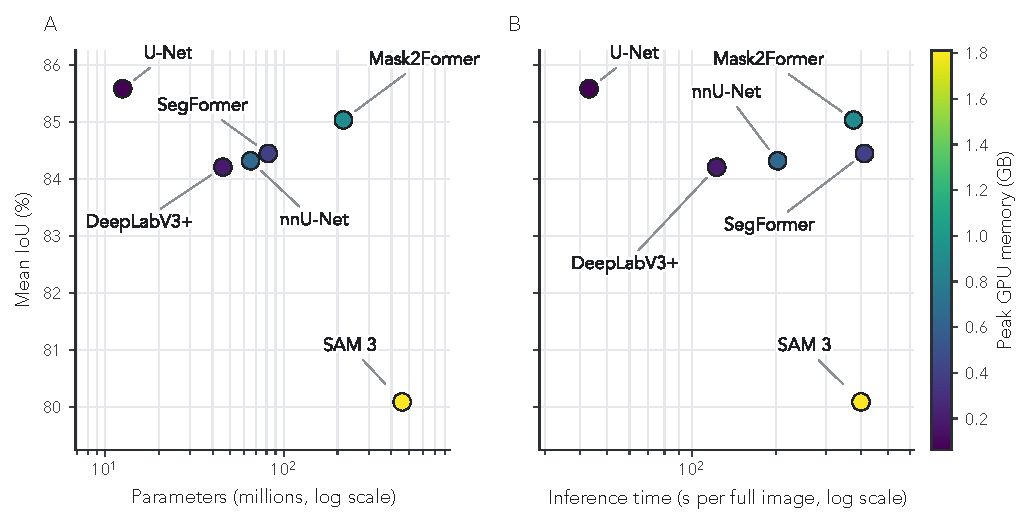
\includegraphics[width=\linewidth]{figures/pennycress-unet/accuracy-efficiency-panels.pdf}
 \captionsetup{justification=raggedright,singlelinecheck=false}
 \caption[Accuracy and computational efficiency of benchmarked segmentation architectures]{Accuracy and computational efficiency of benchmarked segmentation architectures. (A) Best mean IoU (mIoU) achieved by each architecture across its boundary-weighting variants plotted against total parameter count on a log scale. (B) Best mIoU plotted against mean full-image inference time on a log scale, where lower values indicate faster segmentation. Point color and the shared color bar encode peak allocated GPU memory during full-image inference; nnU-Net values were grouped from pod-crop predictions back to the source full images.}
 \label{fig:ch2-accuracy-efficiency}
\end{figure}

We evaluated our models' segmentation performance on 5 raw images containing 65 seed pods in total. Per-class IoU and across-class mIoU are reported in Table~\ref{tab:ch2-pennycress-results}. The boundary down-weighted U-Net achieved the highest mIoU at 85.58\%, narrowly ahead of the baseline U-Net at 85.53\% and Mask2Former at 85.03\%. These top scores were close relative to per-image variation, so we interpret the leading architectures as comparable in accuracy rather than as statistically separable. SAM~3 was the clearest laggard, especially for seed segmentation, where IoU fell as low as 57.61\%.

Efficiency separated the leading architectures more strongly than accuracy (Table~\ref{tab:ch2-efficiency}; Figure~\ref{fig:ch2-accuracy-efficiency}). U-Net used 12.57 million parameters, required 43.1 s per full test image, and peaked at 0.06 GB allocated GPU memory. nnU-Net, DeepLabV3+, SegFormer, Mask2Former, and SAM~3 required more parameters and longer inference times; Mask2Former had a similar mIoU but used 215.45 million parameters, required 377.0 s per full test image, and peaked at 0.90 GB allocated GPU memory. Thus, U-Net provided the most favorable accuracy-efficiency tradeoff for population-scale phenotyping in this small, specialized pod-segmentation task. We found no prior work measuring semantic segmentation of pennycress to compare with our model benchmark suite.

\subsection{Population-Scale Phenotyping}

Having selected U-Net as the most favorable benchmark on accuracy and efficiency, we applied it at population scale to characterize phenotypic structure across the pennycress accession panel. We measured phenotypes from 12,253 seed pods across 768 accessions. Each image yielded approximately 16 retained pod crops on average and took around 2 minutes of model inference time to segment, compared to approximately 1.5 hours of hand segmentation per image, yielding an estimated 30- to 45-fold throughput gain depending on annotator pace.

We used the feature extraction pipeline described in Section~\ref{sec:ch2-phenotype-extraction} to construct an open-source dataset of over 50 phenotypes for all 12,253 seed pods. For visualization and correlation summaries, we excluded detections for which the watershed step returned zero seeds. Figure~\ref{fig:ch2-area-dist} shows the distributions of three key phenotypes: wing area, envelope area, and seed area. These traits correspond directly to the three annotated tissue classes, making their distributions a useful biological plausibility check on segmentation output. Each trait was right-skewed and heavy-tailed, consistent with the log-normal-like distributions commonly observed in quantitative plant traits~\cite{TRY}.

Consistent with the wing-seed regulatory association described in Section~\ref{sec:ch2-pc-background}, wing area was positively correlated with seed area and seed count (Pearson $r = 0.51$ and $0.30$, respectively; Figure~\ref{fig:ch2-wing-seed-corr}). The resulting per-accession phenotype matrix served two roles: as input to iRF-LOOP for PPN construction (Section~\ref{sec:ch2-pen}), and as the candidate trait pool for heritability filtering and GWAS (Section~\ref{sec:ch2-gwas}).

\begin{figure}[!ht]
 \centering
 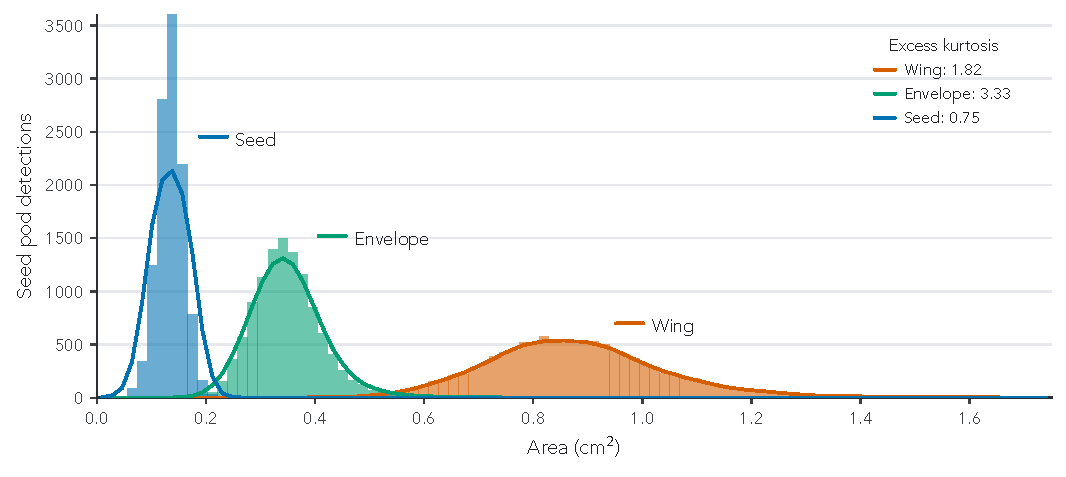
\includegraphics[width=\linewidth]{figures/pennycress-unet/area-distributions.pdf}
 \captionsetup{justification=raggedright,singlelinecheck=false}
 \caption[Distribution of seed-pod component areas]{Distribution of seed-pod component areas across non-empty population-scale detections. Histograms show the measured areas (cm$^2$) of wing, envelope, and seed tissues after excluding detections with zero watershed seed markers. Colored lines show five-bin moving averages of histogram counts, and inset values report excess kurtosis, quantifying heavier-than-normal distribution tails. Seed area is concentrated at smaller values, envelope area at intermediate values, and wing area at larger values; all three traits are right-skewed and log-normal-like, consistent with natural variation in plant morphology.}
 \label{fig:ch2-area-dist}
\end{figure}

\begin{figure}[!ht]
 \centering
 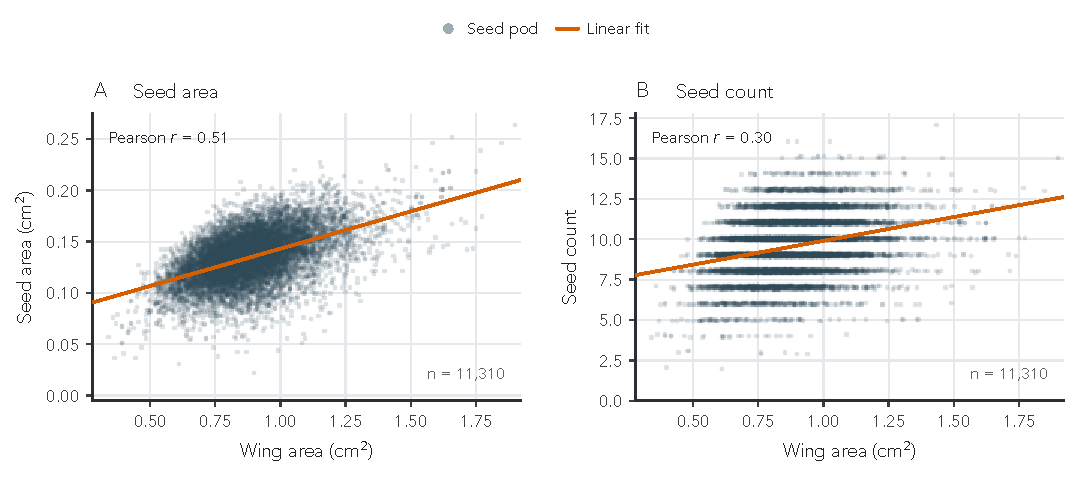
\includegraphics[width=\linewidth]{figures/pennycress-unet/wing-area-v-seed-area-count.pdf}
 \captionsetup{justification=raggedright,singlelinecheck=false}
 \caption[Relationships between wing area and seed traits]{Relationship between wing area and seed traits across non-empty population-scale detections. Wing area is plotted against (A) seed area and (B) seed count, with each point representing one seed pod and the solid line showing the linear least-squares fit. Points in (B) are vertically jittered by less than 0.1 seed for visibility; correlations and fitted lines use the unjittered seed-count values. Wing area is positively correlated with both seed area (Pearson $r = 0.51$) and seed count ($r = 0.30$), consistent with wing--seed regulatory association in \textit{Brassicaceae}.}
 \label{fig:ch2-wing-seed-corr}
\end{figure}

\subsection{Predictive Phenotype Network}
After extracting phenotypes from our dataset, we used iRF-LOOP to construct PPNs to check the biological plausibility of extracted phenotypes. Running iRF-LOOP on the entire dataset yielded a PPN with 48 nodes and 108 directed edges after filtering the network to include only the top 5\% of relationships (Figure~\ref{fig:ch2-pc-ppn}). Despite being a directed network, the PPN exhibited high reciprocity, indicating that predictive relationships tend to be mutual, which is expected for many geometrically derived traits.

\begin{figure}[p]
 \centering
 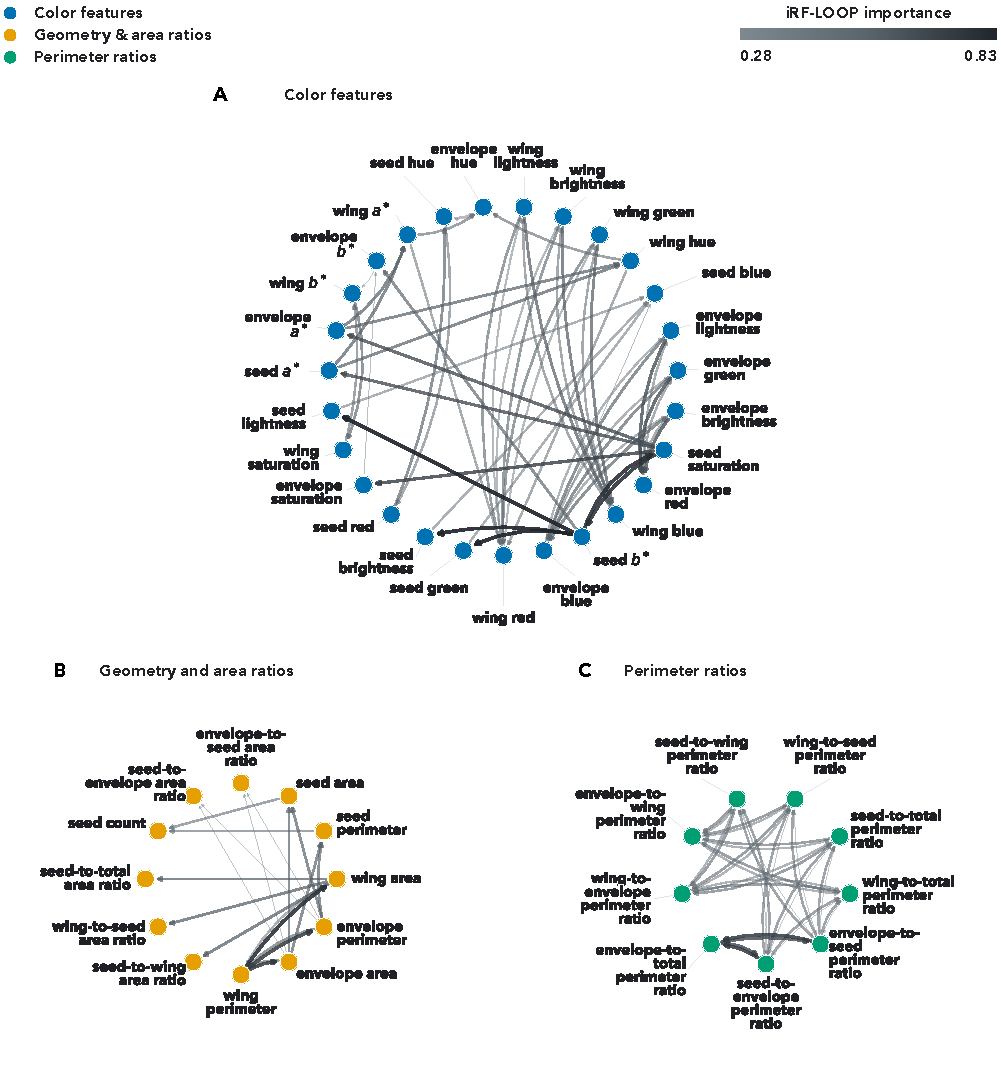
\includegraphics[width=\linewidth]{figures/pennycress-unet/pc-ppn-top0.05.pdf}
 \caption[Predictive phenotype network (PPN) for pod-related traits]{Predictive phenotype network (PPN) for pod-related traits after retaining the top 5\% of iterative Random Forest Leave-One-Out Prediction (iRF-LOOP) relationships. Nodes are measured phenotypes; node color and panel membership denote feature classes: (A) color features, (B) geometry and area ratios, and (C) perimeter ratios. Directed arrows indicate predictor-to-response relationships, and edge width and darkness encode iRF-LOOP importance. The filtered network contains 48 nodes and 108 directed edges. In color-feature labels, $a^*$ and $b^*$ are CIELAB color channels.}
 \label{fig:ch2-pc-ppn}
\end{figure}

The PPN separated into three connected components after filtering, each dominated by a single feature type: a 27-node component containing all color features across all three tissues, a 12-node component containing absolute geometry and area ratios, and a 9-node component containing all perimeter ratios. This separation by measurement type is expected given how tightly color and geometric features covary within each class.

To interpret the cross-tissue relationships more directly, we extracted the subset of PPN edges that connect traits across pod tissues (Figure~\ref{fig:ch2-pc-ppn-focus}). This focused subset separates two recurring patterns: pigment coupling among color traits and size coupling among envelope, seed, and wing geometry traits.

\begin{figure}[p]
 \centering
 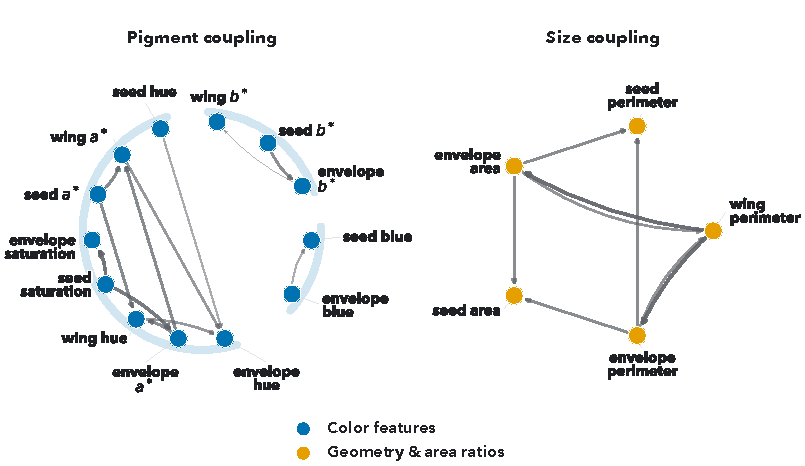
\includegraphics[width=\linewidth]{figures/pennycress-unet/pc-ppn-focus-subset.pdf}
 \captionsetup{justification=raggedright,singlelinecheck=false}
 \caption[Focused subset of cross-tissue predictive phenotype network relationships]{Focused subset of cross-tissue predictive phenotype network relationships. The subset highlights PPN edges connecting traits across pod tissues, separated into pigment coupling and size coupling groups. Nodes are measured phenotypes, with blue nodes denoting color features and orange nodes denoting geometry and area-ratio features. Directed arrows indicate predictor-to-response relationships, and edge width and darkness encode iRF-LOOP importance. Pale blue arcs visually group related pigment-feature relationships. In color-feature labels, $a^*$ and $b^*$ are CIELAB color channels.}
 \label{fig:ch2-pc-ppn-focus}
\end{figure}

Within this focused subset, several informative relationships emerged that could not be explained by geometric identities alone. Most notably, both envelope area and perimeter were predictive of seed area and perimeter (iRF-LOOP importance $\approx 0.56$), consistent with the pod's active role in seed development and resource allocation in \textit{Brassicaceae} \cite{wing-seed-assoc}. This relationship mirrors the envelope-to-seed area ratio, which was the most recurrent of our significant GWAS signals (Section~\ref{sec:ch2-gwas}). Similarly, seed and envelope color features were predictive of each other in CIELAB $b^*$, RGB blue, and HSV hue spaces. This suggests that color features, which provide a proxy for pod maturity and pigmentation, may be co-regulated across tissues. These relationships are correlative and do not imply causality, but they indicate that extracted phenotypes capture biologically coherent structure beyond trivial geometric relationships.

\subsection{Heritability of U-Net-Derived Pod Traits}
Of the 149 phenotypes available for this panel, 52 were extracted by our U-Net pipeline. Screening these for heritable genetic signal retained 34 traits, with $H^2$ ranging from 0.068 to 0.461 (Table~\ref{tab:ch2-heritability}); four of the 34 ultimately yielded significant GWAS associations.

Heritability was strongly structured by trait class. The 19 retained geometry and ratio traits spanned $H^2$ 0.188--0.461, whereas the 15 retained color traits spanned 0.068--0.321, and all seven of the most heritable traits were geometric. The most heritable color trait, wing HSV saturation ($H^2 = 0.321$), fell below every one of them. This separation anticipates the association results below, in which three of the four traits with significant hits are geometry or area ratios.

Heritability was necessary but not sufficient for a GWAS hit, and the retained set includes traits whose genotype variance components were weakly resolved. Fourteen of the 34 retained traits did not reach nominal significance on the restricted likelihood-ratio test ($p > 0.05$), and 12 of those 14 were color traits. Envelope-to-seed area ratio, which produced the most recurrent association signal, was itself borderline ($H^2 = 0.200$, $p = 0.0501$). We therefore treat the downstream candidates as exploratory rather than as well-powered genetic findings. Per-trait $H^2$ for all 52 U-Net-derived traits, including the 18 that fell below the screen, is reported in Table~\ref{tbl:heritability-all}.

\subsection{Genome-Wide Association and Gene Mapping}
We performed GWAS on the U-Net-derived pod traits on a panel of 189 accessions using four GAPIT models (MLM, MLMM, FarmCPU, and BLINK). We retained candidate SNPs with raw-$p < 1 \times 10^{-6}$ (a suggestive association cutoff; a Bonferroni threshold is overly stringent given linkage disequilibrium among SNPs) and MAF $\geq 0.03$, deferring false-positive control to GRIN filtering in the module derivation stage.

GWAS yielded six unique SNPs across four phenotypes: envelope CIELAB $b^*$, envelope-to-seed area ratio, wing area, and wing-to-seed area ratio. The most recurrent signal came from envelope-to-seed area ratio. Our GWAS results are summarized in Table~\ref{tab:ch2-gwas-results}.

\begin{table}[htbp]
 \centering
 \caption[Summary of retained GWAS associations for heritable, U-Net-derived pod traits]{Summary of retained GWAS associations for heritable, U-Net-derived pod traits (dryland environment), tested across 189 genotyped accessions. Associations are reported at a suggestive raw $p < 1\times10^{-6}$ cutoff; linkage disequilibrium among SNPs makes per-SNP tests non-independent, so a Bonferroni threshold is overly conservative. $H^2$, broad-sense heritability; SNPs, number of retained single nucleotide polymorphisms; Models, GAPIT models (MLM, MLMM, FarmCPU, BLINK) producing the associations; Lead SNP, most significant SNP (chromosome\_position); Lead raw $p$, its unadjusted $p$-value.}\label{tab:ch2-gwas-results}
 \small
 \setlength{\tabcolsep}{3.5pt}
 \renewcommand{\arraystretch}{1.1}
 \begin{tabularx}{\textwidth}{@{}>{\raggedright\arraybackslash}p{0.30\textwidth} c c >{\raggedright\arraybackslash}X l c@{}}
 \toprule
 Trait & $H^2$ & SNPs & Models & Lead SNP & Lead raw $p$ \\
 \midrule
 envelope CIELAB $b^*$
 & 0.217 & 1 & MLMM & \texttt{4\_8127381} & $8.71 \times 10^{-7}$ \\

 envelope-to-seed area ratio
 & 0.200 & 3 & BLINK, FarmCPU, MLMM & \texttt{5\_963442} & $1.04 \times 10^{-7}$ \\

 wing area
 & 0.366 & 1 & MLMM & \texttt{7\_63065229} & $4.14 \times 10^{-7}$ \\

 wing-to-seed area ratio
 & 0.285 & 1 & MLMM & \texttt{2\_2343404} & $6.06 \times 10^{-7}$ \\
 \bottomrule
 \end{tabularx}
\end{table}

We mapped the six retained SNPs from GWAS to pennycress genes using the mixed LD-decay and distance-based approach described in Section~\ref{sec:ch2-snp2gene}. For each SNP, we defined a window centered on the SNP with a width set by local LD-decay distance and assigned the annotated genes falling in that window, retaining any gene whose body directly contained that SNP. Windows spanned approximately $24.6$--$49.6$~kb, with strong LD-decay fits ($R^2 = 0.944$--$0.989$), reflecting the different recombination contexts of each chromosomal region. Because all six SNPs yielded reliable LD-decay fits, every candidate gene was assigned from an LD window, and the distance-based fallback was not used.

This procedure produced 69 candidate pennycress genes, with half of the loci tracing to the envelope-to-seed area trait and the remaining loci tracing to the other three GWAS traits. We mapped these genes to their nearest Arabidopsis orthologs in TAIR~\cite{garcia2002tair} to enable cross-species functional annotation and module derivation. This mapping yielded 64 unique orthologs, as several pennycress genes shared a single Arabidopsis ortholog. This ortholog set constitutes the candidate ortholog set carried forward to GRIN filtering and module derivation (Section~\ref{sec:ch2-mentor}).

\subsection{\textsc{Mentor} Module Derivation}
GRIN filtering reduced the candidate ortholog set of 64 genes to 33, pruning 31 that lacked sufficient network support; these 33 constitute the network-supported gene set. We applied \textsc{Mentor} to this set, using the process and standard settings described in Section~\ref{sec:ch2-mentor}, resolving it into three modules of 5, 11, and 17 genes (Figure~\ref{fig:ch2-mentor-dendro}). We then used these modules for mechanistic interpretation (Section~\ref{sec:ch2-mentor-ia}).

\begin{figure}[p]
 \centering
 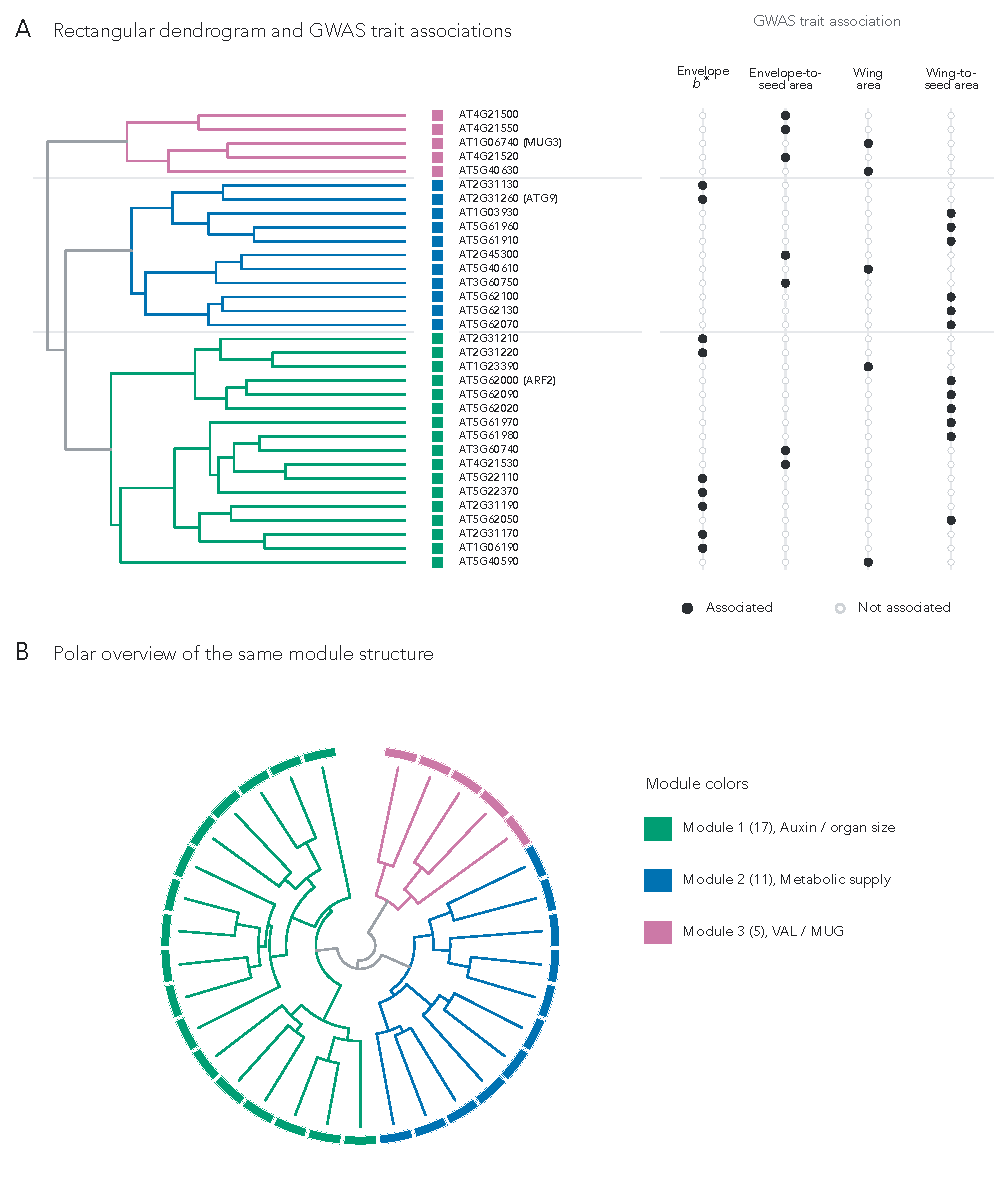
\includegraphics[width=0.96\linewidth,height=0.75\textheight,keepaspectratio]{figures/pennycress-unet/mentor-dendrogram.pdf}
 \caption[\textsc{Mentor} dendrogram of 33 candidate Arabidopsis orthologs retained from U-Net-derived pod traits]{\textsc{Mentor} dendrogram of the 33 GRIN-refined Arabidopsis orthologs retained from U-Net-derived pod-trait GWAS candidates. (A) Complete-linkage clustering of random-walk-with-restart (RWR) dissimilarities, with the adjacent trait matrix indicating which of the four GWAS traits---envelope CIELAB $b^*$, envelope-to-seed area ratio, wing area, and wing-to-seed area ratio---each gene was associated with. (B) Polar view of the same topology, emphasizing the three \textsc{Mentor} modules. Branch and outer-ring colors indicate Module 1 (17 genes; auxin, organ-size, and reproductive development), Module 2 (11 genes; metabolic supply, autophagy, and nutrient remobilization), and Module 3 (5 genes; VAL/MUG transposon-derived regulators).}
 \label{fig:ch2-mentor-dendro}
\end{figure}

\subsection{\textsc{Mentor-IA} Exploratory Interpretation}
We used \textsc{Mentor-IA} to conduct an exploratory interpretation of the three modules derived by \textsc{Mentor} (Section~\ref{sec:ch2-mentor}). Module 1, which contained 17 Arabidopsis orthologs, was run with the enrichment agent, literature agent, mygene interpreter, and meta aggregator. Module 2, which contained 11 orthologs, was run with the same agents as Module 1. Module 3, which contained 5 orthologs, was run with only the mygene interpreter and meta aggregator, as the small gene count limited the power of enrichment analyses. Because our modules did not have an associated network, we did not use the network agent for analysis.

\textsc{Mentor-IA} produced per-agent summaries for each module, along with a final interpretation that synthesized evidence across agents. This interpretation included keyword themes, enrichment statistics from GO and KEGG, and a mechanistic summary with candidate supporting citations. Across modules, the proposed mechanisms recovered known \textit{Brassicaceae} pod and seed biology, demonstrating our pipeline's ability to connect measured phenotypes to candidate mechanistic explanations. We manually cross-checked the agent output against pennycress and \textit{Brassicaceae} literature, finding the mechanistic summaries to be consistent with reported biology.

Because functional interpretation used Arabidopsis orthologs, the mechanisms below should be read as candidate hypotheses rather than validated pennycress-specific effects. For clarity, gene-symbol mentions below refer to Arabidopsis orthologs; parenthetical IDs give the Arabidopsis locus followed by the corresponding pennycress TAV2 locus or loci.

\subsubsection{Module 1 Interpretation}
We confirmed that the \textsc{Mentor-IA} module 1 analysis recovered mechanistic themes centered around auxin-mediated control of organ size and reproductive development, with supporting themes connecting to auxin and cell division more broadly. \cite{schruff2006} demonstrated that Arabidopsis \textit{ARF2} (\texttt{AT5G62000}; pennycress \texttt{TAV2\_LOCUS7857}) represses auxin-responsive transcription, limiting integument cell proliferation, and loss of \textit{ARF2} function leads to enlarged seeds and organs. \cite{paolo2021} found that \textit{ARF2} genetically interacts with \textit{SEEDSTICK} and \textit{GORDITA} during seed development, linking this auxin-response factor to integument growth and seed-coat differentiation. These findings provide the strongest candidate bridge to envelope-to-seed area ratio, while any connection to wing area remains more indirect through broader auxin-mediated organ-growth biology.

Module 1's link to auxin and cell division is further supported by the presence of Arabidopsis \textit{APC4} (\texttt{AT4G21530}; pennycress \texttt{TAV2\_LOCUS24640}), which encodes a subunit of anaphase-promoting complex (APC/C). \cite{wang2012apc4} demonstrated that Arabidopsis \textit{apc4} mutants exhibit defects in female gametogenesis and embryogenesis, with aberrant embryo cell division and distorted auxin distribution. \cite{liu2018arf} also implicated \textit{ARF2}, together with \textit{ARF4} and \textit{ARF5}, in gametophyte development, reinforcing the reproductive-development theme. Arabidopsis \textit{RUS2}/\textit{WXR1} (\texttt{AT2G31190}; pennycress \texttt{TAV2\_LOCUS13944}) provides a second auxin-related but less direct line of evidence. \cite{ge2010} showed that \textit{RUS2}/\textit{WXR1} is required for normal polar auxin transport and PIN/AUX1 abundance in roots, while \cite{leasure2009} placed \textit{RUS2} with \textit{RUS1} in a root UV-B-sensing pathway. Thus, the proposed \textit{RUS2} connection to wing growth is an inference from auxin-distribution biology rather than a demonstrated pod-morphology effect. The module also surfaced a possible connection to color phenotypes such as envelope CIELAB $b^*$; \textit{arf2} mutants show delayed senescence and altered chlorophyll retention in leaves \cite{ellis2005}. Because this evidence comes from leaves and developmental timing instead of pod-envelope color directly, the connection to pod color remains tentative.

In addition to the literature-supported themes that we manually verified, the \textsc{Mentor-IA} enrichment agent returned several significant GO and KEGG terms consistent with reproductive development, such as floral whorl development ($p = 9.8 \times 10^{-5}$), ovule development ($p = 3.6 \times 10^{-3}$), and embryo development ending in seed dormancy ($p = 3.6 \times 10^{-3}$), providing additional support for the proposed developmental theme.

Despite the strong theme and supporting evidence around auxin-mediated control of organ size and reproductive development, the remaining orthologs in module 1 had only gene-level annotation and no clear trait-linking literature in the \textsc{Mentor-IA} output, so we leave their exploration for future work and specify them as additional candidates. The module 1 interpretation is consistent with known biology of pod and seed development in \textit{Brassicaceae}.

\subsubsection{Module 2 Interpretation}
Module 2 is centered around metabolic supply, autophagy, nutrient remobilization, and chloroplast carbon metabolism. Unlike module 1, which provides evidence of a direct developmental regulator in \textit{ARF2}, module 2 provides an indirect hypothesis in which metabolic supply from the pod to the seed may influence pod growth. The strongest candidate connection is to envelope-to-seed area ratio and pod filling because the literature links these pathways to seed resource allocation rather than directly to pod morphology.

Arabidopsis \textit{ATG9} (\texttt{AT2G31260}; pennycress \texttt{TAV2\_LOCUS12330}) anchors the module's autophagy signal. \cite{shin2014} showed that \textit{ATG9} contributes to autophagic flux, while \cite{inoue2006} found that \textit{atg9} mutants retain constitutive autophagy in root tips, supporting a modulatory role instead of a strictly essential one. \cite{kang2018} and \cite{luo2023} place \textit{ATG9} in autophagosome formation and closure pathways, and \cite{lai2020} provides structural evidence for \textit{ATG9}'s role in autophagy via cryo-EM, showing that it is the core integral membrane autophagy protein. \cite{guiboileau2012} observed that \textit{atg} mutants show reduced nitrogen remobilization to seeds under both low- and high-nitrate conditions, and \cite{diberardino2018} demonstrated that autophagy affects resource allocation and storage-protein accumulation during seed development. These findings suggest that variation in autophagy may affect pod filling or envelope-to-seed nutrient allocation, providing a candidate link to phenotypes like envelope-to-seed area ratio.

Arabidopsis \textit{TKL1} (\texttt{AT3G60750}; pennycress \texttt{TAV2\_LOCUS16016}) provides a second line of evidence for metabolic supply and chloroplast carbon metabolism. \cite{rocha2014} found that \textit{TKL1} is phosphorylated at Ser428 in a light- and chloroplast-dependent manner, suggesting that it may be a regulatory point for carbon flux in the Calvin-Benson-Bassham (CBB) cycle and oxidative pentose phosphate pathway (OPPP). Additionally, \cite{khozaei2015} demonstrated that altered plastid transketolase dosage disrupts growth through thiamine- and TPP-related metabolic constraints. Because carbon supply is important to seed growth, we infer that \textit{TKL1} may provide a second, indirect link to pod growth and envelope-to-seed area, supporting our mechanistic supply hypothesis.

Additionally, \cite{shen2006} adds a redox-homeostasis line of evidence, showing that Arabidopsis \textit{GPDHc1} (\texttt{AT5G40610}; pennycress \texttt{TAV2\_LOCUS25599}) controls plant NADH/NAD\textsuperscript{+} ratios through the mitochondrial glycerol-3-phosphate shuttle. Although the OPPP is not directly implicated in this work, it supports a broader interpretation in which module 2 captures genes involved in carbon and redox balance during pod and seed development.

Outside of the autophagy and metabolic supply themes, the remaining module 2 genes had only gene-level annotation and no clear trait-linking literature, so we specify them as additional candidates for future exploration. Overall, the module 2 interpretation is consistent with known biology of seed filling and envelope-to-seed biomass allocation, providing a plausible but indirect mechanistic hypothesis connecting our phenotypes to metabolic supply and autophagy.

\subsubsection{Module 3 Interpretation}
Since module 3 yielded only sparse gene-level annotation and lacked enrichment and literature support, we did not advance a mechanistic interpretation for it; its genes remain candidates for future analysis.

\subsubsection{Expression-Based Plausibility Check}
We further evaluated the plausibility of our candidate mechanisms by examining gene expression in pennycress leaf, pod, and root tissues using the dataset from \cite{combsgiroir2024waterlogging}. For the purpose of connecting candidate genes to pod phenotypes, we focused on expression in pod tissues. The strongest literature-supported candidate loci were expressed in pods. These included the module 1 candidates \textit{ARF2} (\texttt{TAV2\_LOCUS7857}), \textit{APC4} (\texttt{TAV2\_LOCUS24640}), and \textit{RUS2} (\texttt{TAV2\_LOCUS13944}), and the module 2 candidates \textit{ATG9} (\texttt{TAV2\_LOCUS12330}), \textit{TKL1} (\texttt{TAV2\_LOCUS16016}), and \textit{GPDHc1} (\texttt{TAV2\_LOCUS25599}). By contrast, several lower-priority candidate loci were not highly expressed in pod tissues. The \textit{BAG2} orthologs were \texttt{TAV2\_LOCUS6658} and \texttt{TAV2\_LOCUS26197}. The \textit{bHLH010} ortholog was \texttt{TAV2\_LOCUS13948}; the \textit{bHLH091} orthologs were \texttt{TAV2\_LOCUS13945} and \texttt{TAV2\_LOCUS13946}. These lower expression patterns support our focus on the literature-backed mechanisms. The sparse expression of many module 3 paralogs also supports treating that module as a future-work candidate set. Overall, expression results indicate that prioritized candidates are active in pod tissues, supporting their plausibility as candidate mechanisms and providing a basis for future experimental validation.

\begin{figure}[p]
 \centering
 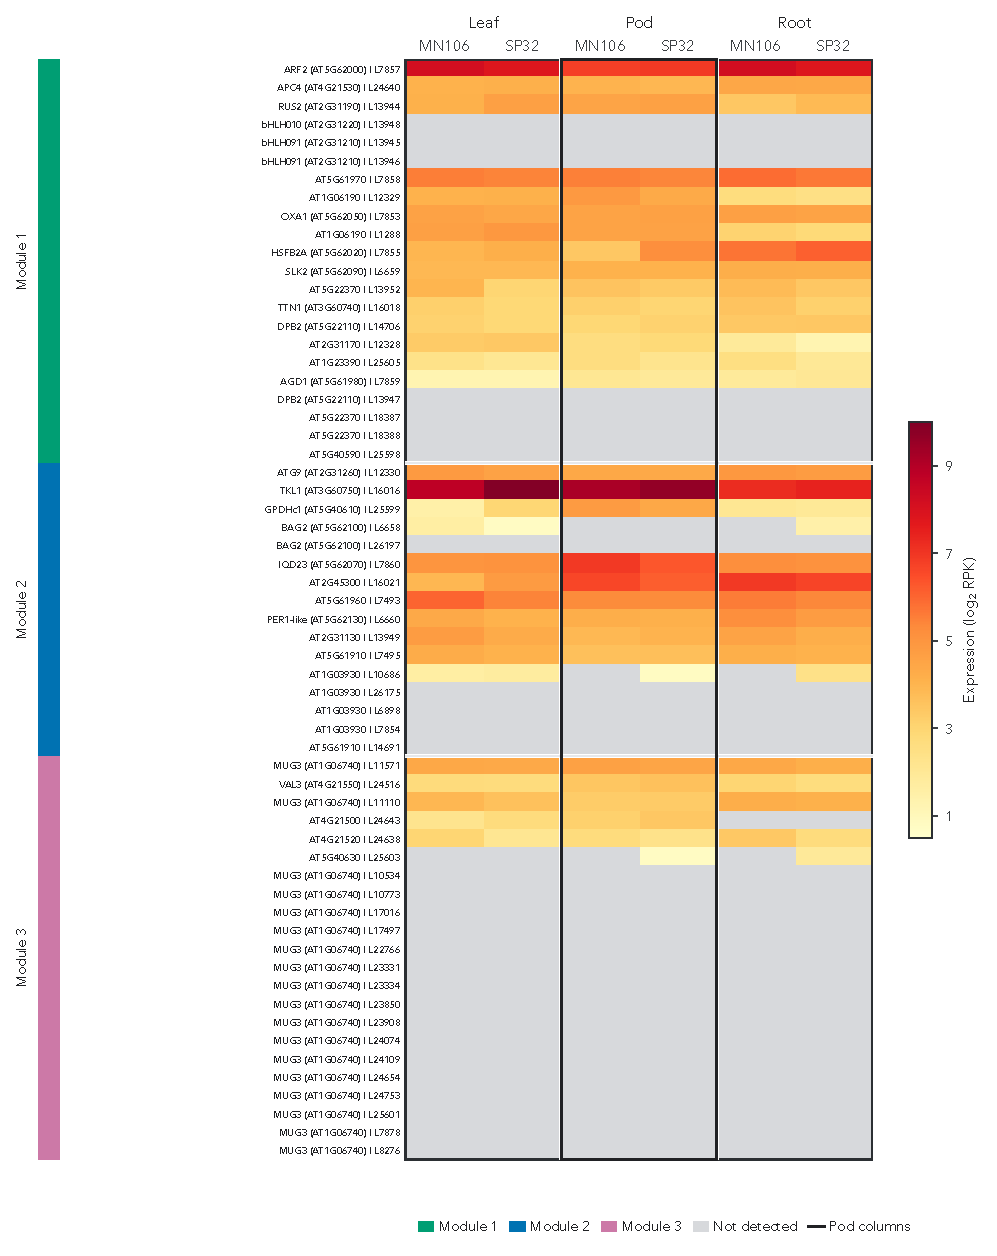
\includegraphics[width=\linewidth,height=0.76\textheight,keepaspectratio]{figures/pennycress-unet/pod-expression-heatmap.pdf}
 \captionsetup{justification=raggedright,singlelinecheck=false}
 \caption[Expression of \textsc{Mentor}-derived candidate loci across pennycress tissues]{Expression of \textsc{Mentor}-derived candidate loci across pennycress tissues. Rows are pennycress loci grouped by \textsc{Mentor} module; repeated Arabidopsis orthologs reflect paralogous pennycress loci. Cell color encodes log$_2$-transformed expression (reads per kilobase) in leaf, pod, and root tissue for MN106 and SP32, with gray cells denoting values below the detection threshold ($\leq 0.5$). Pod columns are grouped and outlined because the candidate-gene plausibility assessment focuses on pod expression, and bold row labels mark literature-supported candidates emphasized in the text.}
 \label{fig:ch2-combined-expression}
\end{figure}

\section{Discussion}
We found that a custom U-Net provided the most favorable accuracy-efficiency tradeoff among the benchmarked CNN, transformer, and foundation model architectures when training and testing on our open-source, hand-annotated ground truth dataset of 347 seed pod images. These results suggest that for small, specialized biological datasets like ours, a task-specific CNN with tailored inductive biases can match or modestly exceed more complex architectures while requiring less computation. However, we note that our small dataset size and tiling scheme may have limited the performance of transformer- and foundation model-based architectures, which rely on large receptive fields and pretraining priors. Future work could explore whether larger datasets and different preprocessing strategies can unlock the potential of these architectures for pennycress phenotyping.

Our pipeline produced 52 biologically plausible, tissue-resolved phenotypes at population scale (12,253 seed pods over 768 accessions). Deep learning methods provided a 30- to 45-fold speedup over manual annotation while achieving 85.58\% mIoU. Extracted seed, wing, and envelope areas exhibited a log-normal distribution, wing area was positively correlated with seed area and count, and the resulting PPN separated into coherent color, geometry, and perimeter sub-networks while highlighting cross-tissue pigment and size coupling. These results indicate that our pipeline may enable new avenues for research on pennycress seed pod biology through accurate and fast high-throughput measurements.

Starting from our image-derived pod traits, our pipeline surfaced candidate genes and mechanisms that recover known \textit{Brassicaceae} pod and seed biology. GWAS yielded significant associations for four pod traits, which we mapped to 69 pennycress genes and 64 Arabidopsis orthologs. GRIN narrowed these to 33 network-supported candidates, which \textsc{Mentor} resolved into three modules; two were related to pod and seed biology. Module 1 was the strongest, centered on auxin-mediated organ growth, reproductive development, and cell division. Its key gene, \textit{ARF2}, offers the clearest candidate bridge to envelope-to-seed area. Module 2 was more indirect: autophagy, nutrient remobilization, and redox balance via \textit{ATG9}, \textit{TKL1}, and \textit{GPDHc1} support a plausible metabolic-supply hypothesis for pod filling and envelope-to-seed allocation. However, these candidates rest on Arabidopsis orthologs, as pennycress network and literature data remain limited.

We compared the \textsc{Mentor-IA} results to pennycress gene expression data, using the expression heatmap to assess hypothesis plausibility in pod tissues. Prioritized Module 1 and 2 candidates were expressed in pods, while some lower-priority candidates were weakly expressed or not detected, supporting our focus on the literature-backed mechanisms. Furthermore, Module 3 expression is sparse, supporting our decision to treat it as a candidate set for future work. It is important to note that expression was measured across the whole pod and is correlative, so it does not establish causality or eQTL regulation. However, our expression evidence supports prioritization of our literature-backed candidates for future studies.

Despite this progress, our work has some limitations. Collecting and scanning seed pods to use for segmentation is still a labor-intensive process; this could become a bottleneck in future population-scale studies, and it only yielded a small training set. Additionally, the model's performance is dependent on the quality of label data due to its supervised nature. Accurately annotating seed border pixels was difficult due to the low brightness and contrast levels in image scans, and this limitation was reflected in the lower accuracy for seeds than other surfaces. Furthermore, benchmark compatibility with nnU-Net is imperfect due to its built-in adaptive preprocessing and evaluation pipeline.

Additionally, GWAS results are limited as they used only 189 accessions and retained SNPs with a permissive threshold, although GRIN did help filter candidates further. Due to the limited availability of pennycress data, we relied on Arabidopsis orthologs for module derivation and interpretation, which may not fully capture pennycress biology. Finally, the \textsc{Mentor-IA} interpretation is exploratory and based on literature evidence from Arabidopsis, so it must be experimentally validated in pennycress to draw strong conclusions.

We present several avenues for future work to extend this pipeline. Improving imaging quality and scanning throughput could yield higher-quality datasets, which can also be expanded through more hand annotation for ground truth. Additionally, performing GWAS on a larger panel of accessions can provide higher-powered association results. Finally, experimental validation of the candidate mechanisms, such as \textit{ARF2}/\textit{APC4}/\textit{RUS2} and \textit{ATG9}/\textit{TKL1}/\textit{GPDHc1}, can test their relevance to pennycress pod phenotypes and provide a deeper understanding of the underlying biology.

This work has several implications for future pennycress research. We found no prior work that extracts intensive phenotypes from pennycress seed pods due to the labor-intensive nature of this task. Therefore, this article provides a novel pipeline for extracting several biologically important phenotypes at the population scale for pennycress and linking them to genetic variants. The framework allows scientists to perform experiments on pennycress that were previously impossible; for example, researchers can examine how treatments and experimental conditions affect entire populations by measuring seed pod phenotypes across treatment groups. Furthermore, scientists can test hypotheses about phenotypic relationships on a broad scale, leading to higher-impact research. More broadly, this work shows how deep learning-derived phenotypes can be carried into genetic association and module-level interpretation to prioritize table biological hypotheses.
